\documentclass{article}
\usepackage[utf8]{inputenc}
\usepackage{graphicx}
\usepackage{amsmath}
\usepackage{geometry}
\geometry{a4paper, margin=1in}
\usepackage{booktabs}
\usepackage{threeparttable}
\usepackage{tabularx}
\usepackage{array}
\usepackage{setspace}
\usepackage{parskip}
\usepackage{microtype}
\usepackage[hidelinks]{hyperref}
\usepackage{caption}
\usepackage{fancyhdr}
\usepackage{float}

% ----netlogo code chunk design----
% ---------------------------------
\usepackage{listings}
\usepackage{xcolor}

% Define NetLogo language colors
\definecolor{netlogo_comment}{RGB}{128, 128, 128} % Gray for comments
\definecolor{netlogo_keyword}{RGB}{0, 0, 204}    % Blue for structural keywords
\definecolor{netlogo_command}{RGB}{102, 0, 153}  % Purple for commands
\definecolor{netlogo_string}{RGB}{153, 0, 0}     % Dark red for strings

% Custom NetLogo language definition
\lstdefinelanguage{NetLogo}{
  % Structural keywords
  morekeywords={to, end, extensions, globals, breed, turtles-own, patches-own, links-own}, 
  % Primary commands
  morekeywords=[2]{ask, tick, setup, go, update-plots, create-turtles, hatch, sprout, move-to, forward, fd, back, bk, left, lt, right, rt, set, let, ifelse, if, while, repeat, stop, report}, 
  % Agents and variables
  morekeywords=[3]{turtles, patches, links, world-width, world-height, count, any?, all?, one-of, n-of, with, neighbors, neighbors4}, 
  sensitive=false,
  morecomment=[l]{;}, % NetLogo uses semicolon for comments
  morestring=[b]",    % Strings are enclosed in double quotes
  basicstyle=\ttfamily\small,
  keywordstyle=\color{netlogo_keyword}\bfseries,
  keywordstyle=[2]\color{netlogo_command},
  keywordstyle=[3]\color{teal},
  commentstyle=\color{netlogo_comment}\itshape,
  stringstyle=\color{netlogo_string},
  breaklines=true,
  frame=single,
  numbers=left,
  numberstyle=\tiny\color{gray}
}
% ---------------------------------
% ---------------------------------

\newcolumntype{Y}{>{\centering\arraybackslash}X}
\setstretch{1.15}

\pagestyle{fancy}

\fancyhf{}
\rhead{\small CASA0011 --- Systematic Experimentation (SugarScape)}
\cfoot{\small\thepage}
\renewcommand{\headrulewidth}{0.4pt}

\title{
    \vspace{2cm}
    \Huge \textbf{Agent-Based Modeling --- Coursework 1} \\[0.5cm]
    \large CASA0011 --- Systematic Experimentation (SugarScape)\\[0.5cm]
    \Large \textit{Evolutionary Dynamics of Market Competition: \\ From Individual Survival to Corporate Expansion} \\[1.5cm]
    
    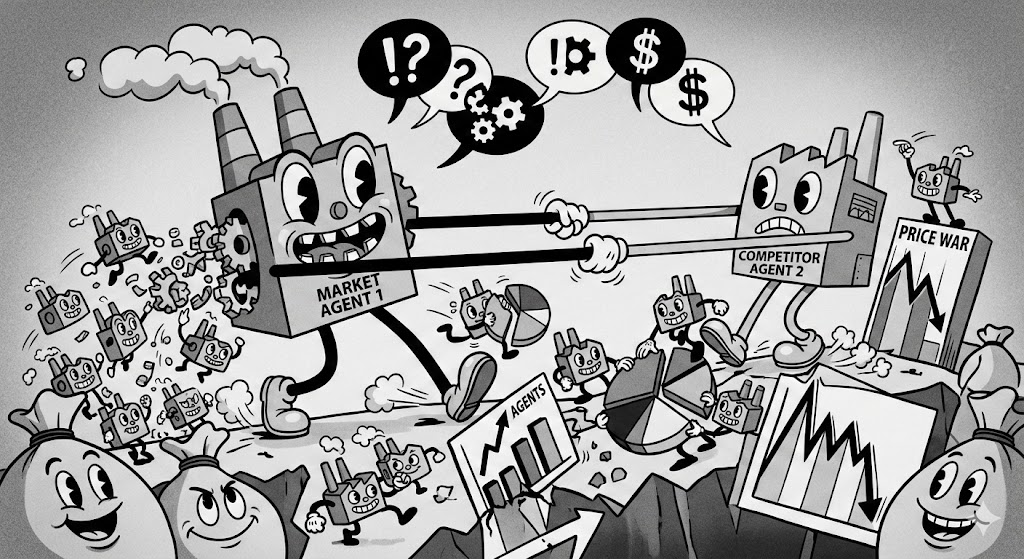
\includegraphics[width=0.85\textwidth]{cover.jpg} \\[1cm]
}

\author{
    \Large \textbf{Zhengpei Xu} \\[0.3cm]
    \large Student Number: 25034404 \\[0.3cm]
}

\date{
    \vfill
    \large March 2026 \\[0.3cm]
    \normalsize Word Count: 1493
}

\begin{document}
\maketitle
\thispagestyle{empty}
\newpage
\pagenumbering{arabic}

% ============================================================
% 0. BACKGROUND 
% ============================================================
\section{Background}
The SugarScape model (Epstein and Axtell, 1996) was originally designed to simulate how complex social phenomena emerge from simple interactions among heterogeneous individuals competing for limited resources. The model series can also be applied in market competition context. Park et al. (2024) adapted the SugarScape framework in a housing market to study how agents’ demand and limited vision decide market outcomes. Based on this, this study extends the model to firm-level competition.





% ============================================================
% 1. AIM 
% ============================================================
\section{Aim}

This study reinterprets the SugarScape model 2 (Constant Growback) and 3 (Wealth Distribution) from the NetLogo Library (Wilensky, 1999a, 1999b) as models of firm-level market competition. In this context, I translate metabolism into operating costs, vision into market awareness, and accumulated sugar into retained capital. Then two progressive stages are designed to examine how market structure and competitive pressure jointly shape firm characteristics and market inequality. Research questions are set below:

\textbf{Stage A (based on Model 2):} In a static and resource-limited market, how does firm density reshape the distribution of firm characteristics through competition?

\textbf{Stage B (based on Model 3):} In a dynamic market with a brand expansion mechanism, how entry conditions for opening branch shape market structure through a filtering process. Does efficiency gain from enterprise scaling further concentrate wealth among dominant brands, creating a winner-takes-more market dynamic? 

Together, the two stages form a progressive comparative framework from static competition to dynamic expansion.

% ============================================================
% 2. METHOD (446 words)
% ============================================================
\section{Method}
This study enhances two SugarScape models and conducts systematic parameter experiments with Netlogo BehaviorSpace. To ensure selection is entirely through market competition rather than lifespan randomness of the initial model, bankruptcy (retained capital falling to zero) is set as the exit mechanism for both. 

To observe and compare cross-stage market resource absorption efficiency, I introduce market utilization ($U$) as a common benchmark in the two stages, which is defined as follows:

\begin{equation}
    U\footnote{In the Stage B secondary experiment, $U$ exceeding 100\% is because the introduction of the same-brand adjacency efficiency mechanism ($b$) improves firms' actual harvesting efficiency.} = \frac{\sum \text{operating cost of all firms}}{\sum \text{sugar regrown across all patches}} \times 100\%
\end{equation}





\subsection{Stage A: Static Competitive Market}

Stage A extends the SugarScape 2 Constant Growback model with two additional reporters: market utilization and Gini Index\footnote{The Gini Index measures wealth inequality within a population, ranging from 0 (perfect equality, all firms hold equal wealth) to 1 (perfect inequality, one firm holds all wealth). A higher value indicates greater wealth concentration.} (measuring wealth distribution). The initial number of firms $N$ (market density) is the sole independent variable. Observed metrics are mean operating cost, mean market reach, market utilization, and Gini Index. Experimental parameters are detailed in Table~1.

\subsection{Stage B: Dynamic Expansion Market}

The original SugarScape 3 reproduction mechanism replaces each dying agent with a single offspring in the same location, modelling biological succession rather than organisational growth. Stage B replaces it with a brand expansion mechanism, where wealthy firms open new branches within their own market reach. The new branding mechanism comprises four rules: 

\begin{enumerate}
    \item When a firm’s wealth exceeds the expansion threshold ET, it attempts to open a new branch each tick with probability $p$.
    
    \item The parent firm transfers a random amount drawn from  $[\text{MW}, \text{ET}]$ (where MW is the minimum entry wealth and ET is the expansion threshold) to the new branch, reducing its own wealth accordingly.
    
    \item The new branch inherits the parent's brand identity, draws operating cost and market reach independently from the same initial distributions, and is placed on a random vacant patch within the parent's market reach (vision) range.
    
    \item If a firm has at least one same-brand neighbour (up/down/left/right), its actual harvested is $S'_i = S_i \times (1 + b)$, where $b$ is the adjacent harvest bonus and $b = 0$ represents the no-scale-effect baseline.
\end{enumerate}
With brand feature introduced, the only wealth distribution measurement Gini Index is not enough. Brand-level Gini reporter is added to the model, forming a dual-layer inequality measurement system.

The experiment is conducted through two sub-stages. The primary experiment adopts a full factorial design across ET and MW to examine the interaction effects of entry conditions. The secondary experiment fixes ET and MW and sweeps Adjacency Harvest Bonus (b) to isolate the effect of scale efficiency on market structure. Observed metrics across both experiments are mean operating cost, mean market reach, market utilization, individual-level Gini Index, and brand-level Gini Index. Full parameters are detailed in Table~1.



\subsection{Stages Experiments Parameter Summary}

\begin{table}[H]
\begin{threeparttable}
\centering
\caption{Experiment Parameter Summary}
\begin{tabularx}{\textwidth}{lXXX}
\toprule
\textbf{Stage} & \textbf{Parameter(s)} & \textbf{Values Tested} & \textbf{Fixed Parameters} \\
\midrule
\multicolumn{4}{l}{\textit{Universal constants: operating cost $\sim U(1,4)$, market reach $\sim U(1,6)$, sugar growback $= 1$}} \\
\midrule
A --- Model 2 & Initial number of firms $N$ (market density) & 10--2499 (15 levels, density-stratified sampling) & initial capital $\sim U(5,25)$ \\
\addlinespace
B --- Model 3 (primary) & Expansion threshold (ET) $\times$ Minimum entry wealth (MW) & ET: $\{10,20,30,40,50\}$; MW: $\{0,9,19,29,39,49\}$; ET $>$ MW (20 valid combinations) & $N=400$, $p=0.6$, $b=0$ \\
\addlinespace
B --- Model 3 (secondary) & Adjacency harvest bonus $b$ & 0--1.0 (step $= 0.1$) & $N=400$, $p=0.6$, ET $=20$, MW $=10$ \\
\bottomrule
\end{tabularx}
\begin{tablenotes}
\small
\item \parbox{\dimexpr\textwidth-2em}{\textit{Note: All experiments were repeated 30 times. Stage A ran for 500 steps and Stage B for 1000 steps; pre-experiments confirm all parameter combinations reach steady state within these limits. Stage A adopts density-stratified sampling: $N \in \{10, 50, 100, 200, 300, 400, 600, 800, 1000, 1200, 1400, 1600, 1800, 2000, 2200, 2499\}$, with finer intervals at low density ($N < 200$) to capture early competitive selection dynamics, and $N = 2499$ included to observe market behaviour at the firm population ceiling. MW is designed as $\{0, 9, 19, 29, 39, 49\}$ so that each ET level includes an MW $=$ ET$-1$ case, capturing the effect of a near-zero startup capital range. Branching probability $p = 0.6$ is validated by pre-experiments to ensure market convergence within the time limit and treated as a control parameter.}}
\end{tablenotes}
\end{threeparttable}
\end{table}



% ============================================================
% 3. RESULTS
% ============================================================
\section{Results}

\subsection{Stage A}

\begin{figure}[H]
    \centering
    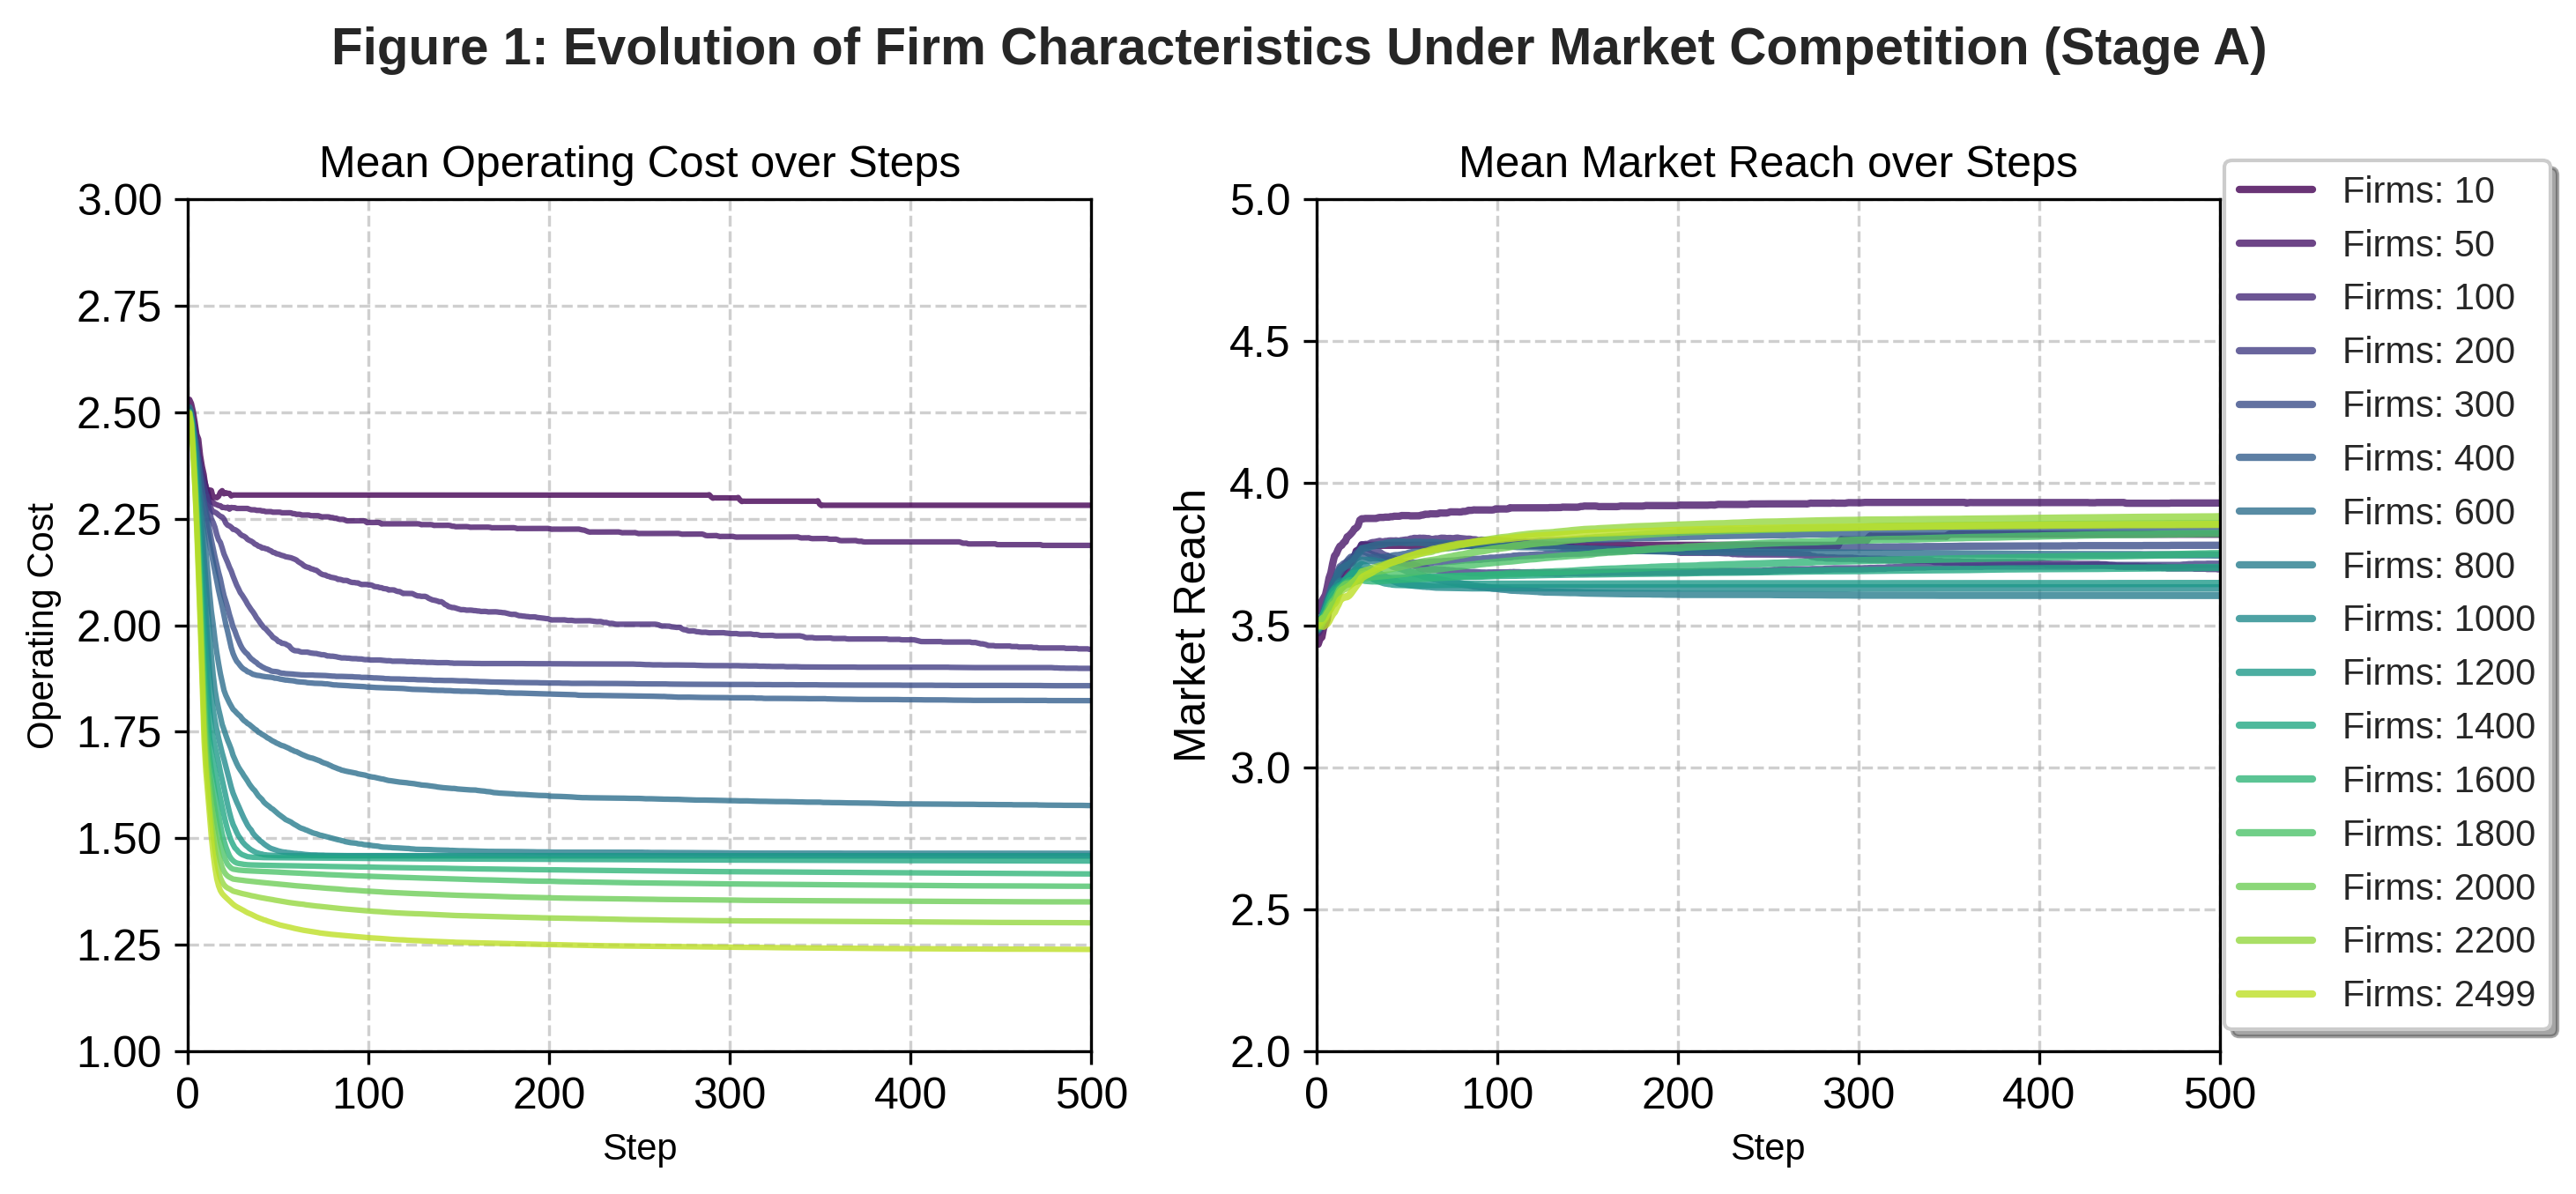
\includegraphics[width=1\linewidth]{stage_A_1.png}
\end{figure}

Figure 1 shows mean operating cost declining nonlinearly from approximately 2.3 to 1.25 as $N$ increases. Mean market reach decreases first and then slightly increases, reaching its minimum when $N = 800$. Figure 2 compares standard deviation bands at three density levels. At $N = 10$, the range of dispersion in operating costs and market reach is extremely wide. As market density increases, both metrics become stable.

\begin{figure}[H]
    \centering
    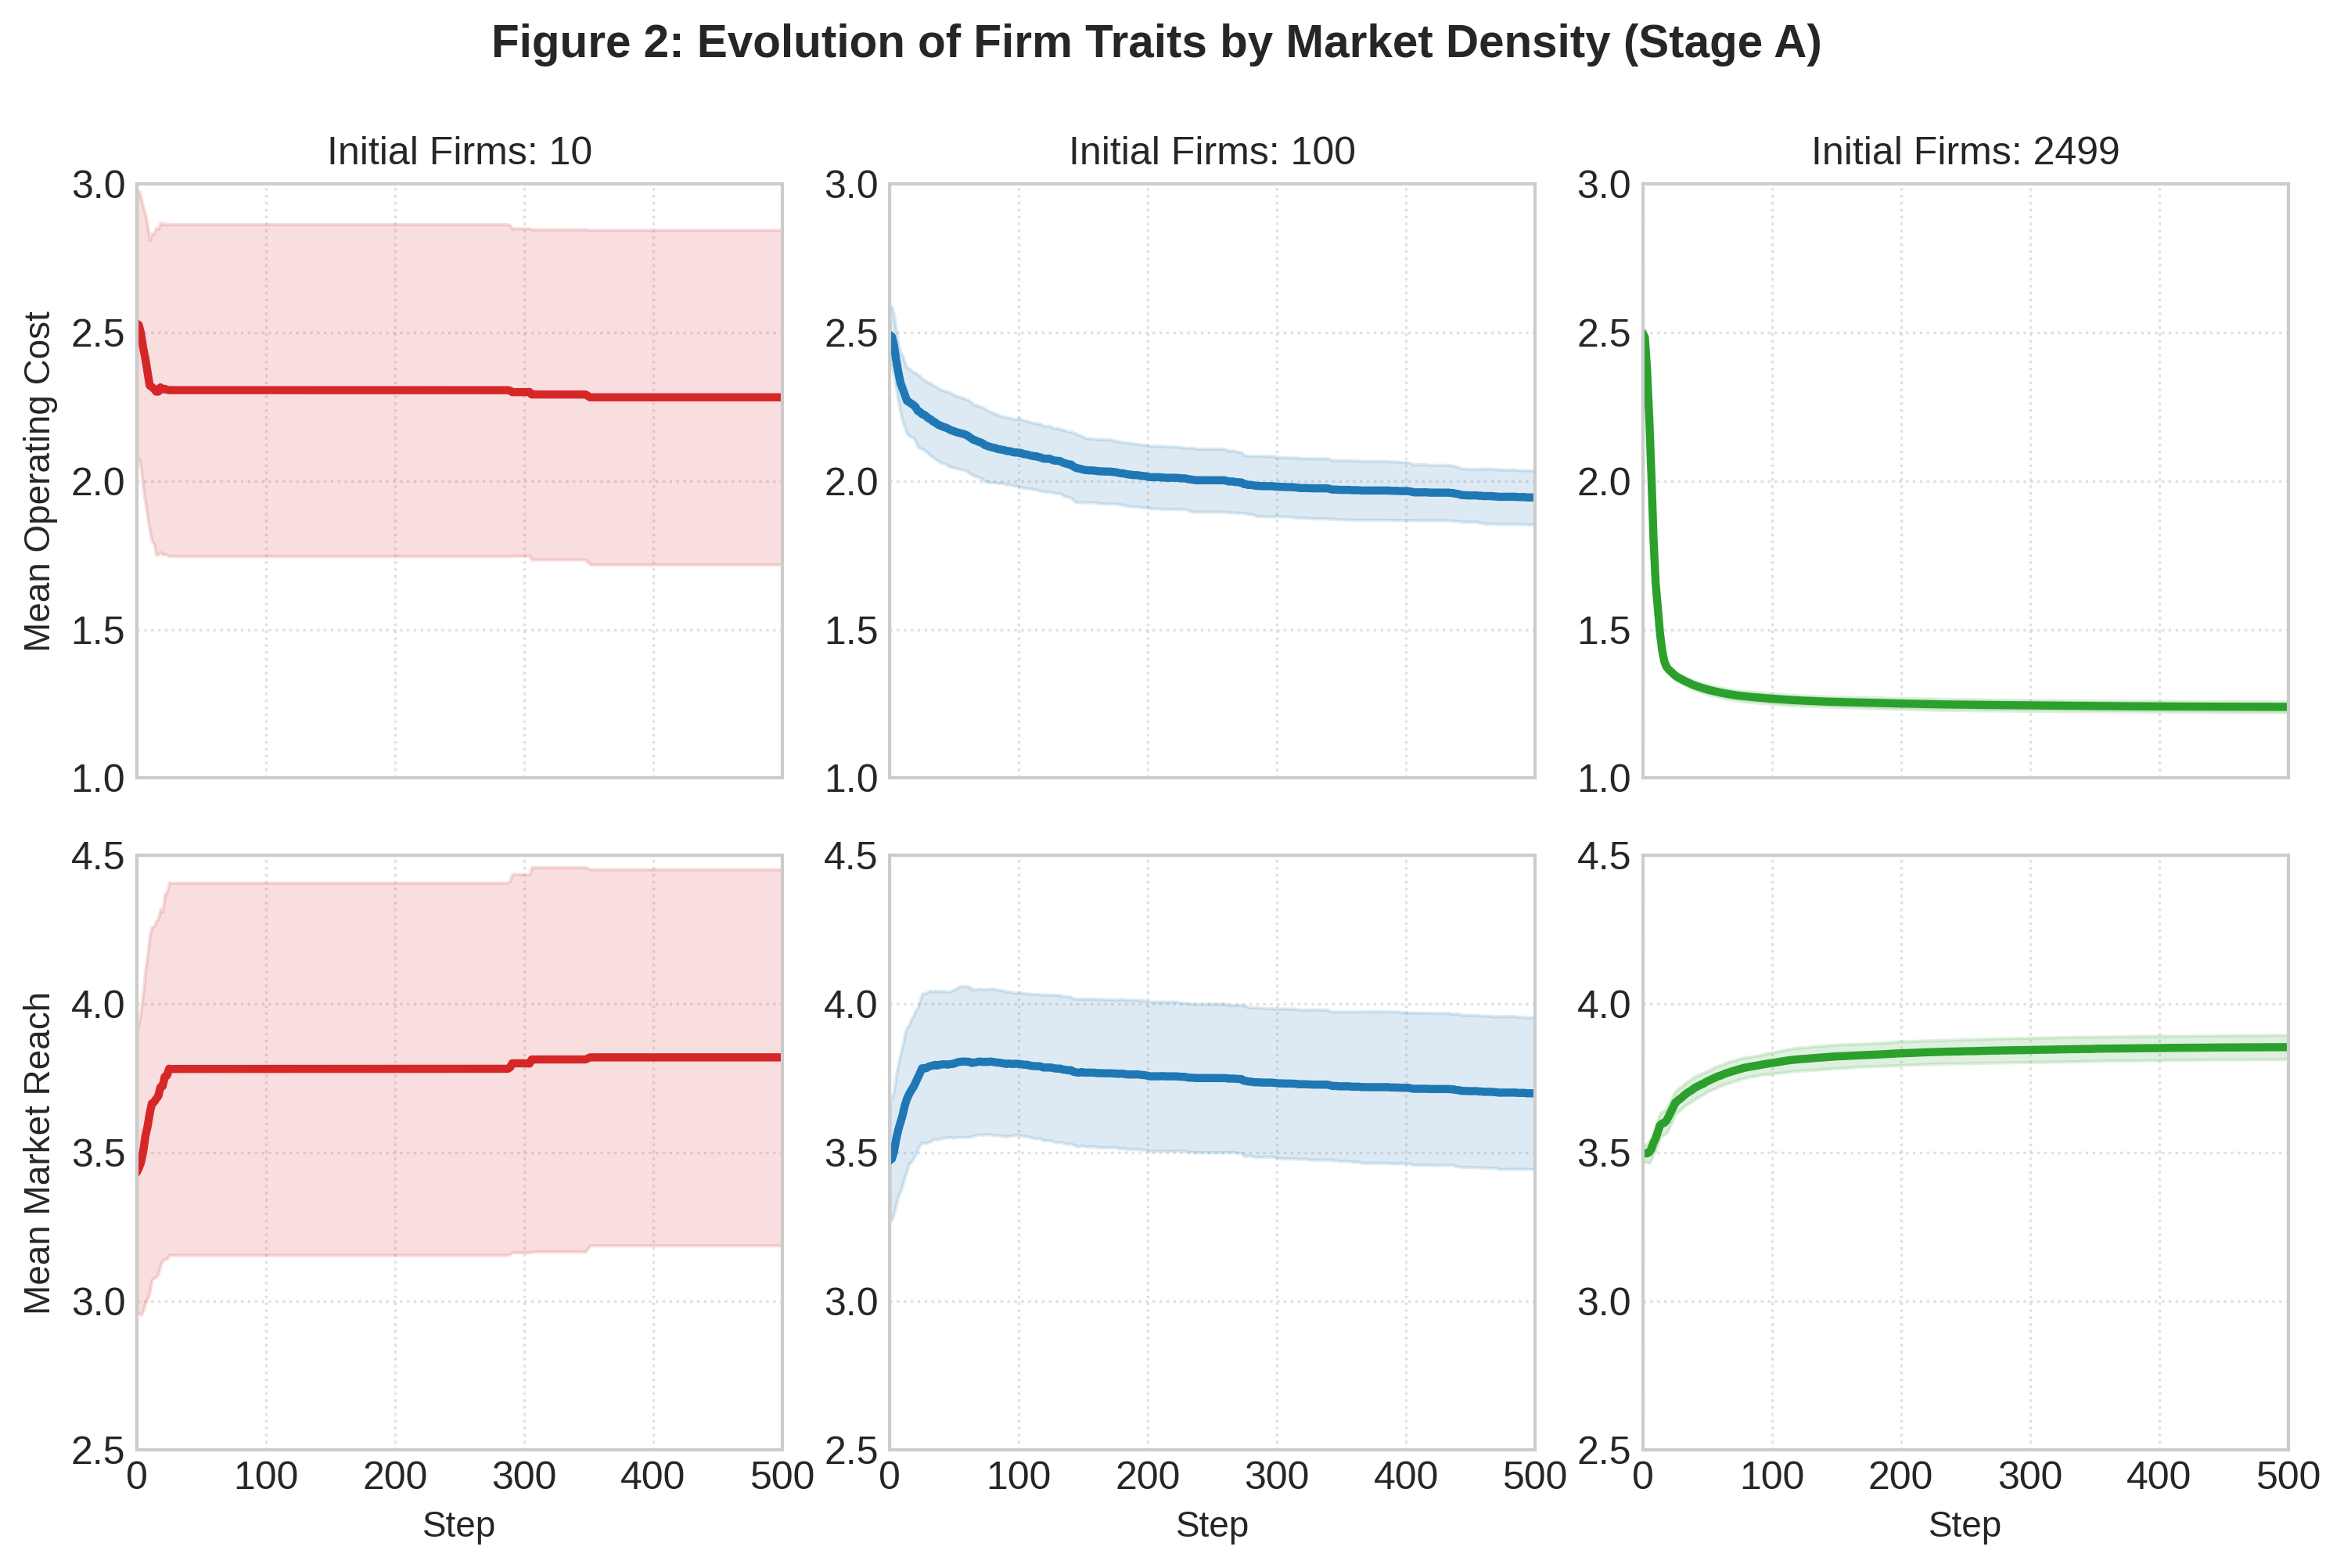
\includegraphics[width=1\linewidth]{stage_A_2.png}
\end{figure}

Figure 3 shows market utilization rising continuously with $N$, reaching 47.14\% at $N = 2000$. Utilization fails to increase further even at the model ceiling of $N = 2499$, indicating a structural ceiling on resource absorption.



\begin{figure}[H]
    \centering
    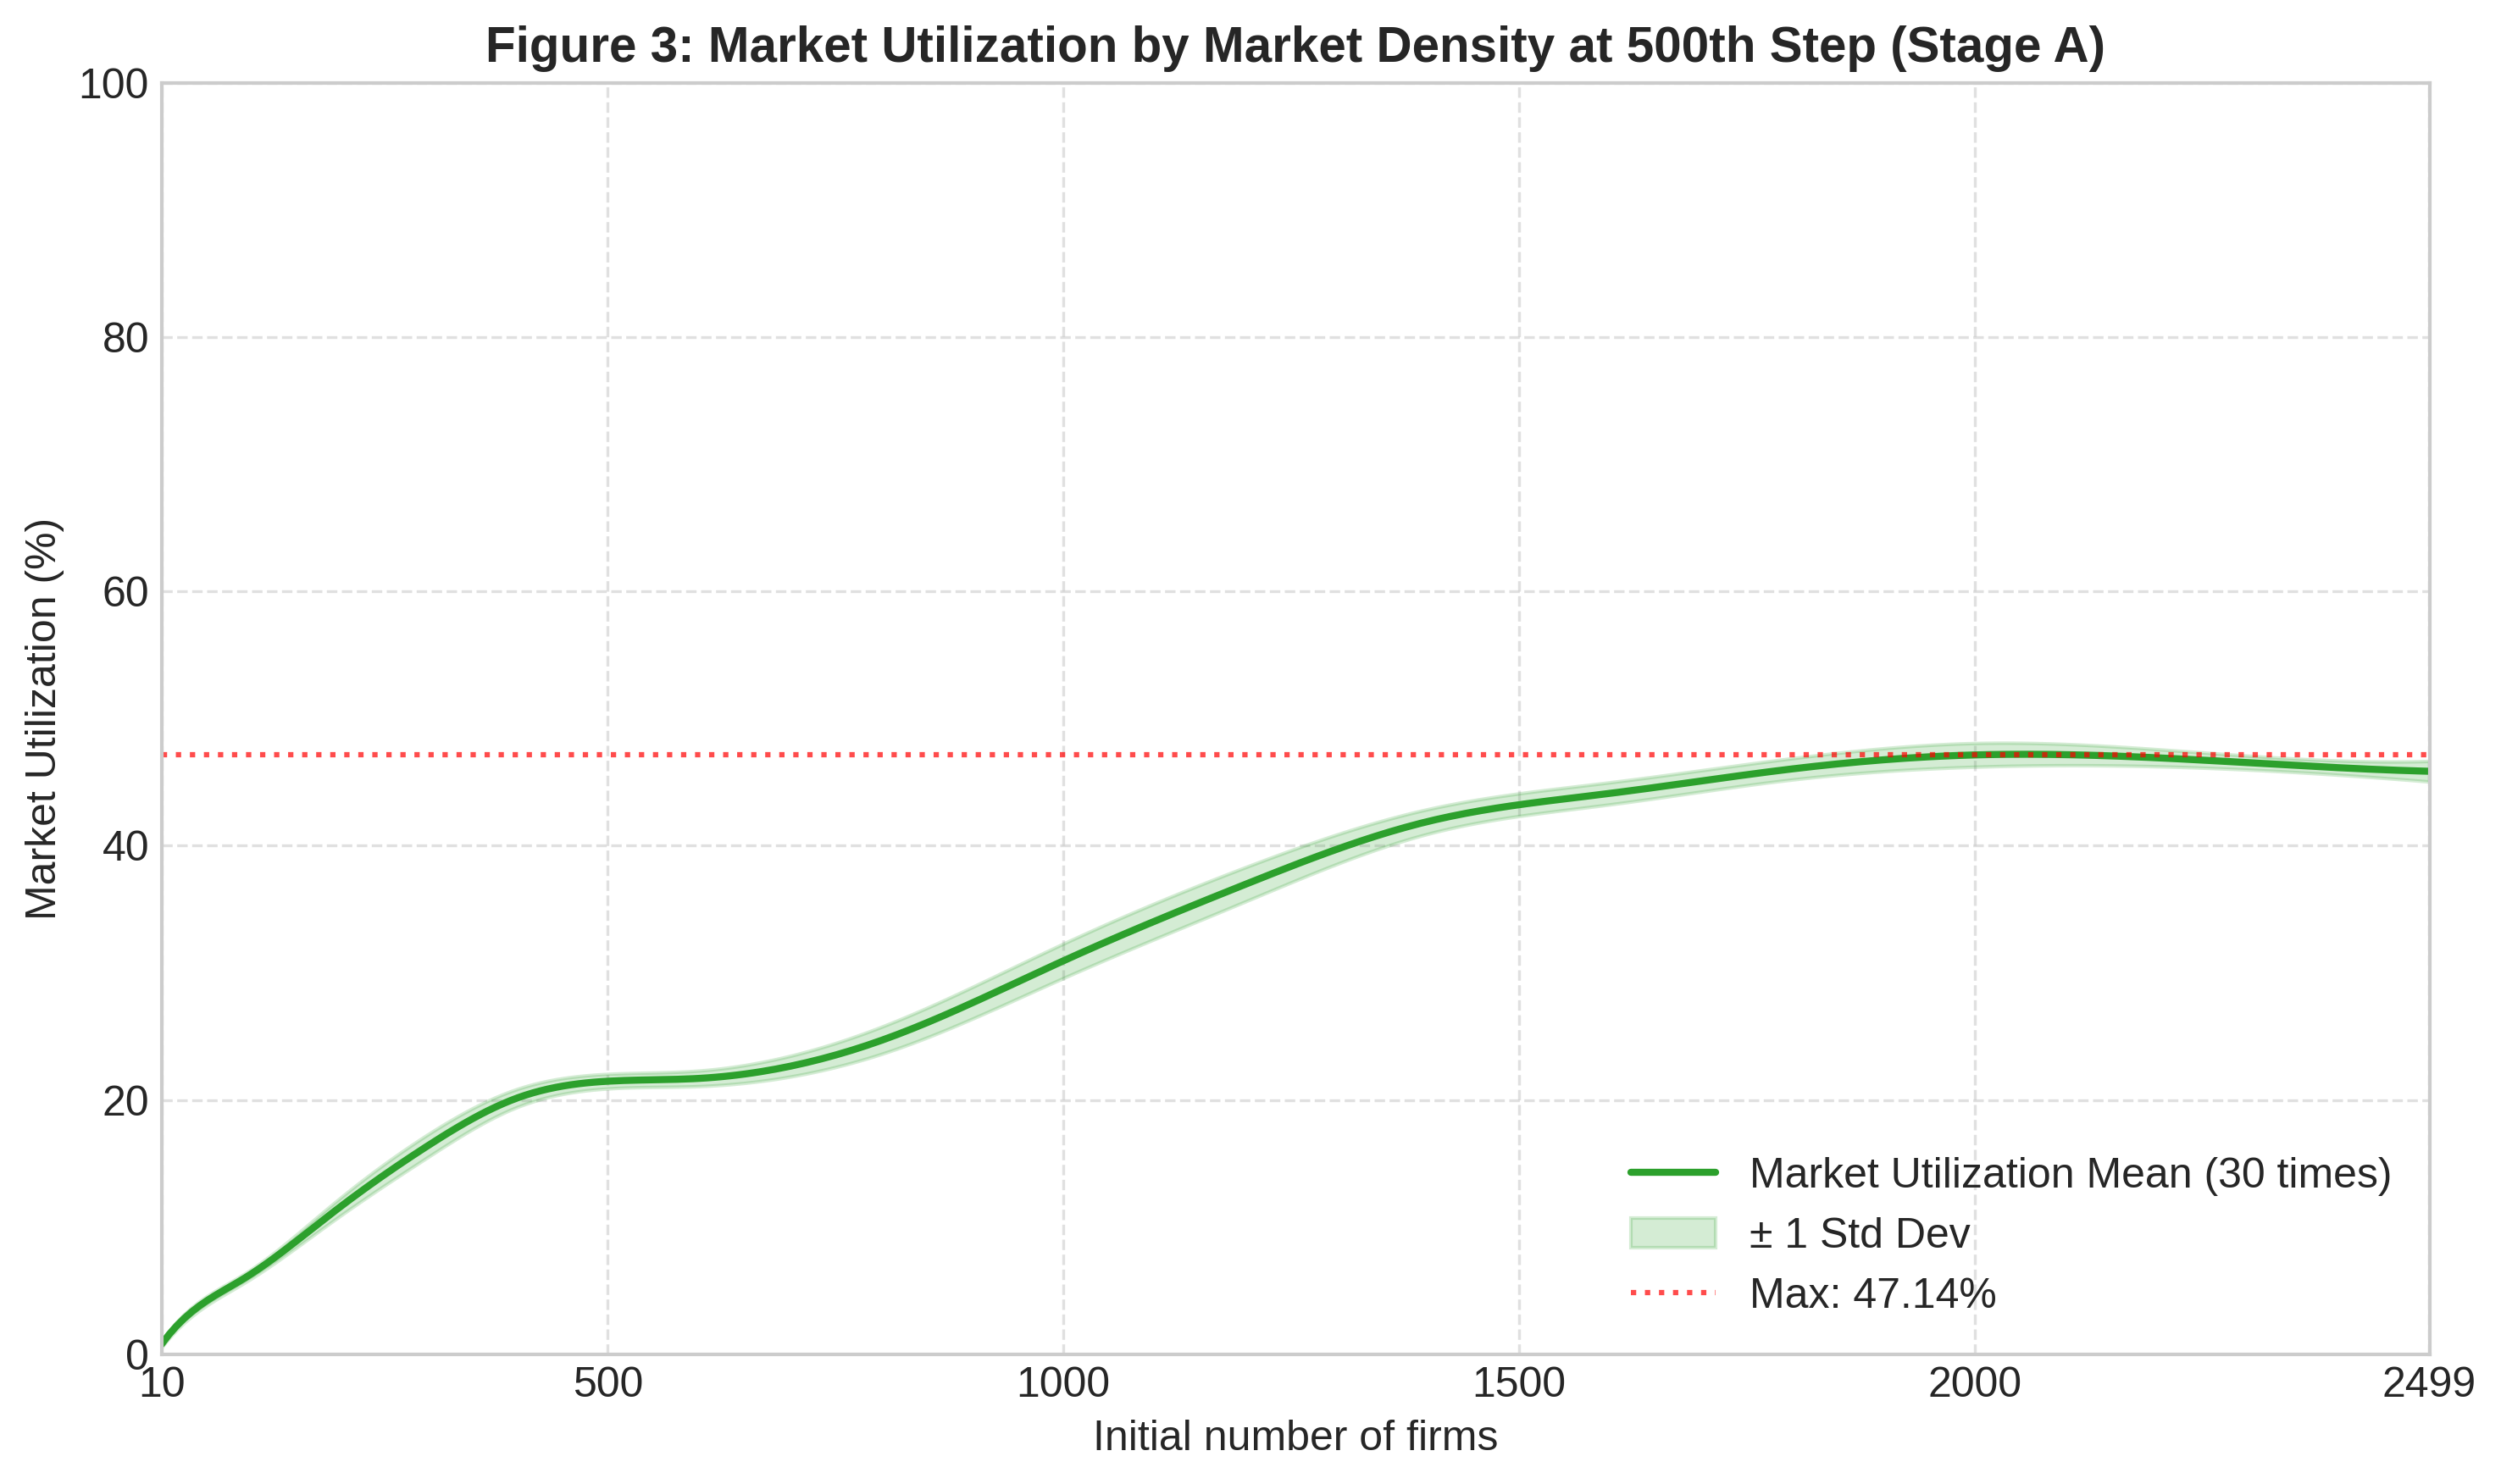
\includegraphics[width=1\linewidth]{stage_A_3.png}
\end{figure}

\begin{figure}[H]
    \centering
    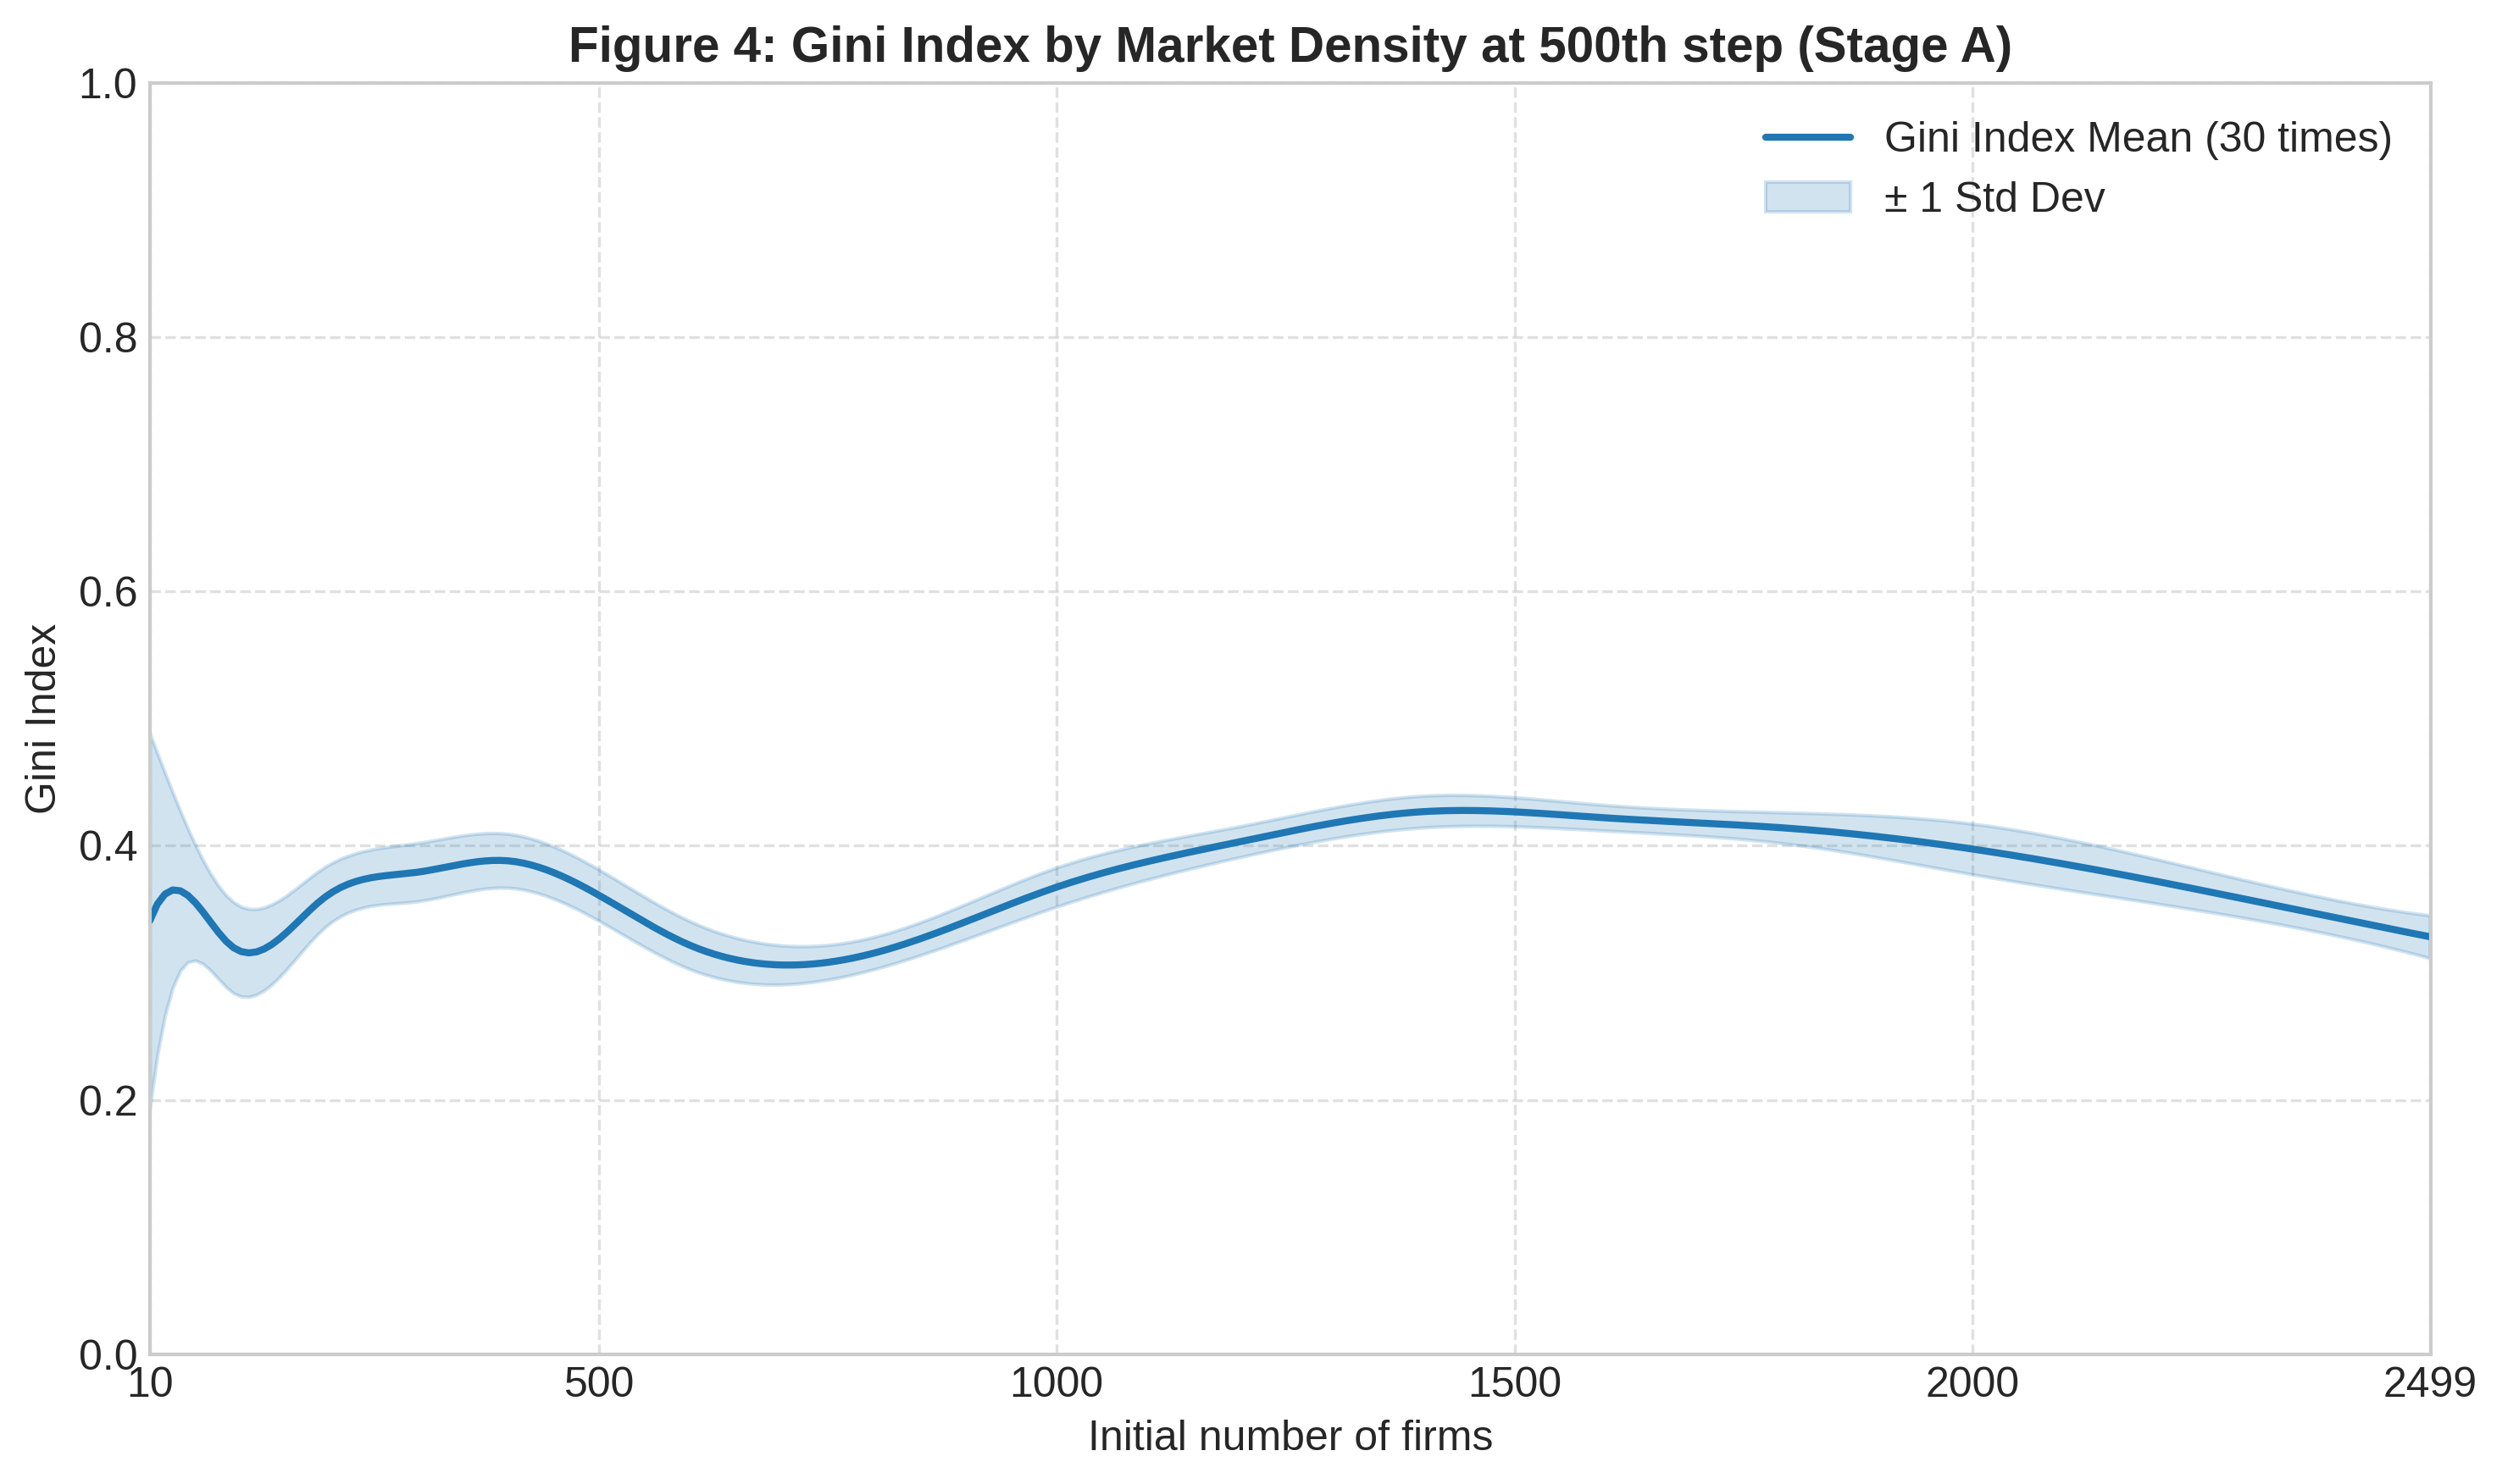
\includegraphics[width=1\linewidth]{stage_A_4.png}
\end{figure}

Figure 4 shows the Gini Index following a non-monotonic pattern. When $N < 100$, the standard deviation range is wide, reflecting highly random outcomes. The Gini then declines to approximately 0.30 at $N = 800$, peaks at 0.43 around $N \approx 1400$, and falls to approximately 0.33 at higher densities.

When N = 800, resource-rich patches begin to saturate, marking a transition from cost-based to location-based selection. Below this threshold, competitive pressure is insufficient to eliminate high-cost firms; above it, positional advantage dominates survival outcomes. This explains why N = 800 coincides with the minimum values of both the Gini Index and mean market reach.


\subsection{Stage B --- Primary Experiment (ET $\times$ MW)}







\begin{table}[H]
\begin{threeparttable}
\centering
\caption{Mean Market Reach (Vision) by Entry Conditions (ET $\times$ MW), mean $\pm$ std}
\label{tab:vision}
\begin{tabularx}{\textwidth}{cYYYYYY}
\toprule
\textbf{ET $\backslash$ MW} & \textbf{0} & \textbf{9} & \textbf{19} & \textbf{29} & \textbf{39} & \textbf{49} \\
\midrule
\textbf{10} & $3.50\pm0.04$ & $3.50\pm0.05$ & --- & --- & --- & --- \\
\textbf{20} & $3.50\pm0.06$ & $3.50\pm0.04$ & $3.51\pm0.04$ & --- & --- & --- \\
\textbf{30} & $3.51\pm0.05$ & $3.50\pm0.05$ & $3.48\pm0.06$ & $3.52\pm0.05$ & --- & --- \\
\textbf{40} & $3.52\pm0.05$ & $3.51\pm0.04$ & $3.50\pm0.04$ & $3.51\pm0.04$ & $3.52\pm0.03$ & --- \\
\textbf{50} & $3.51\pm0.03$ & $3.50\pm0.04$ & $3.49\pm0.04$ & $3.49\pm0.03$ & $3.53\pm0.05$ & $3.52\pm0.04$ \\
\bottomrule
\end{tabularx}
\begin{tablenotes}
\small
\item \textit{Note: Cells marked ``---'' represent invalid combinations where ET $\leq$ MW. All values rounded to 2 decimal places.}
\end{tablenotes}
\end{threeparttable}
\end{table}

\begin{table}[H]
\begin{threeparttable}
\centering
\caption{Mean Operating Cost (Metabolism) by Entry Conditions (ET $\times$ MW), mean $\pm$ std}
\label{tab:metabolism}
\begin{tabularx}{\textwidth}{cYYYYYY}
\toprule
\textbf{ET $\backslash$ MW} & \textbf{0} & \textbf{9} & \textbf{19} & \textbf{29} & \textbf{39} & \textbf{49} \\
\midrule
\textbf{10} & $1.000\pm0.000$ & $1.000\pm0.000$ & --- & --- & --- & --- \\
\textbf{20} & $1.000\pm0.000$ & $1.000\pm0.000$ & $1.000\pm0.001$ & --- & --- & --- \\
\textbf{30} & $1.000\pm0.000$ & $1.001\pm0.001$ & $1.001\pm0.001$ & $1.004\pm0.002$ & --- & --- \\
\textbf{40} & $1.001\pm0.001$ & $1.003\pm0.002$ & $1.006\pm0.003$ & $1.009\pm0.003$ & $1.018\pm0.005$ & --- \\
\textbf{50} & $1.004\pm0.002$ & $1.006\pm0.003$ & $1.015\pm0.004$ & $1.023\pm0.006$ & $1.034\pm0.005$ & $1.044\pm0.007$ \\
\bottomrule
\end{tabularx}
\begin{tablenotes}
\small
\item \textit{Note: Cells marked ``---'' represent invalid combinations where ET $\leq$ MW. Bold indicates the maximum observed deviation from the model floor. All values rounded to 3 decimal places.}
\end{tablenotes}
\end{threeparttable}
\end{table}

Tables 2 and 3 show mean market reach stable at $3.50 \pm 0.05$ and mean operating cost converging to the model floor of 1.00 under most conditions.

\begin{figure}[H]
    \centering
    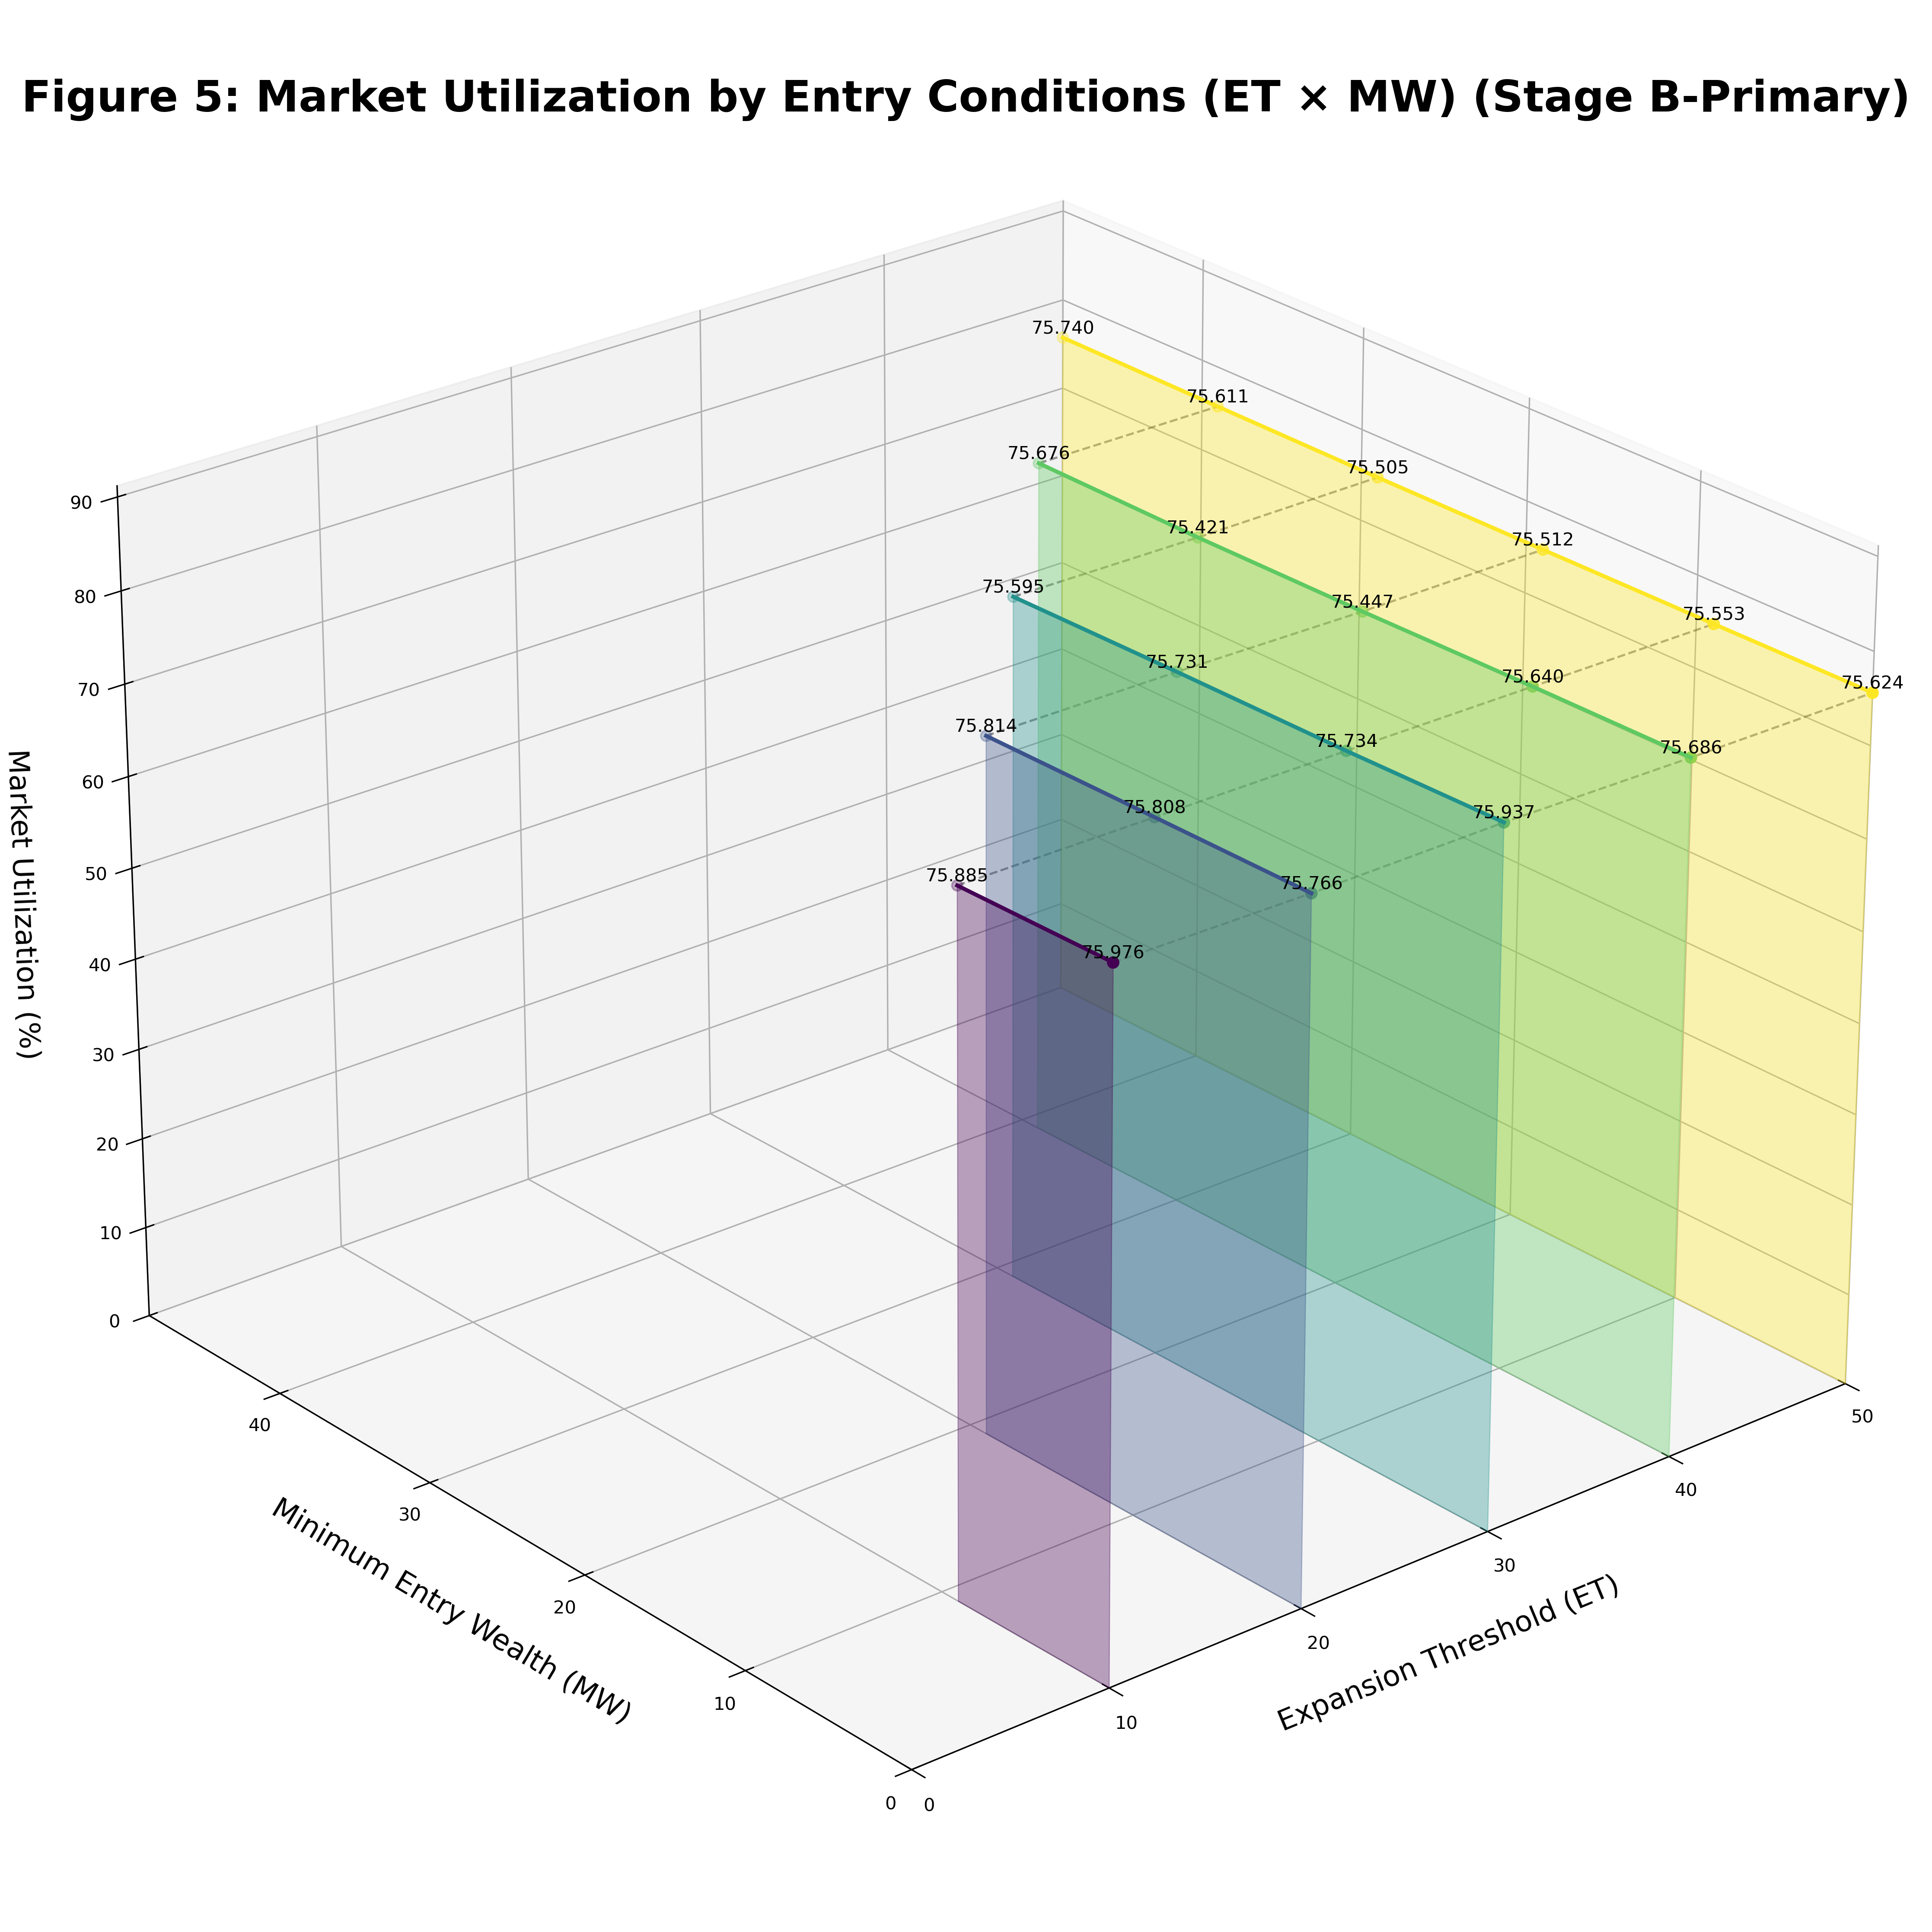
\includegraphics[width=0.75\linewidth]{stage_B_1_1.png}
\end{figure}

Figure 5 shows market utilization is similarly insensitive to ET and MW, staying between 75.4\% and 76.0\%.

\begin{figure}[H]
    \centering
    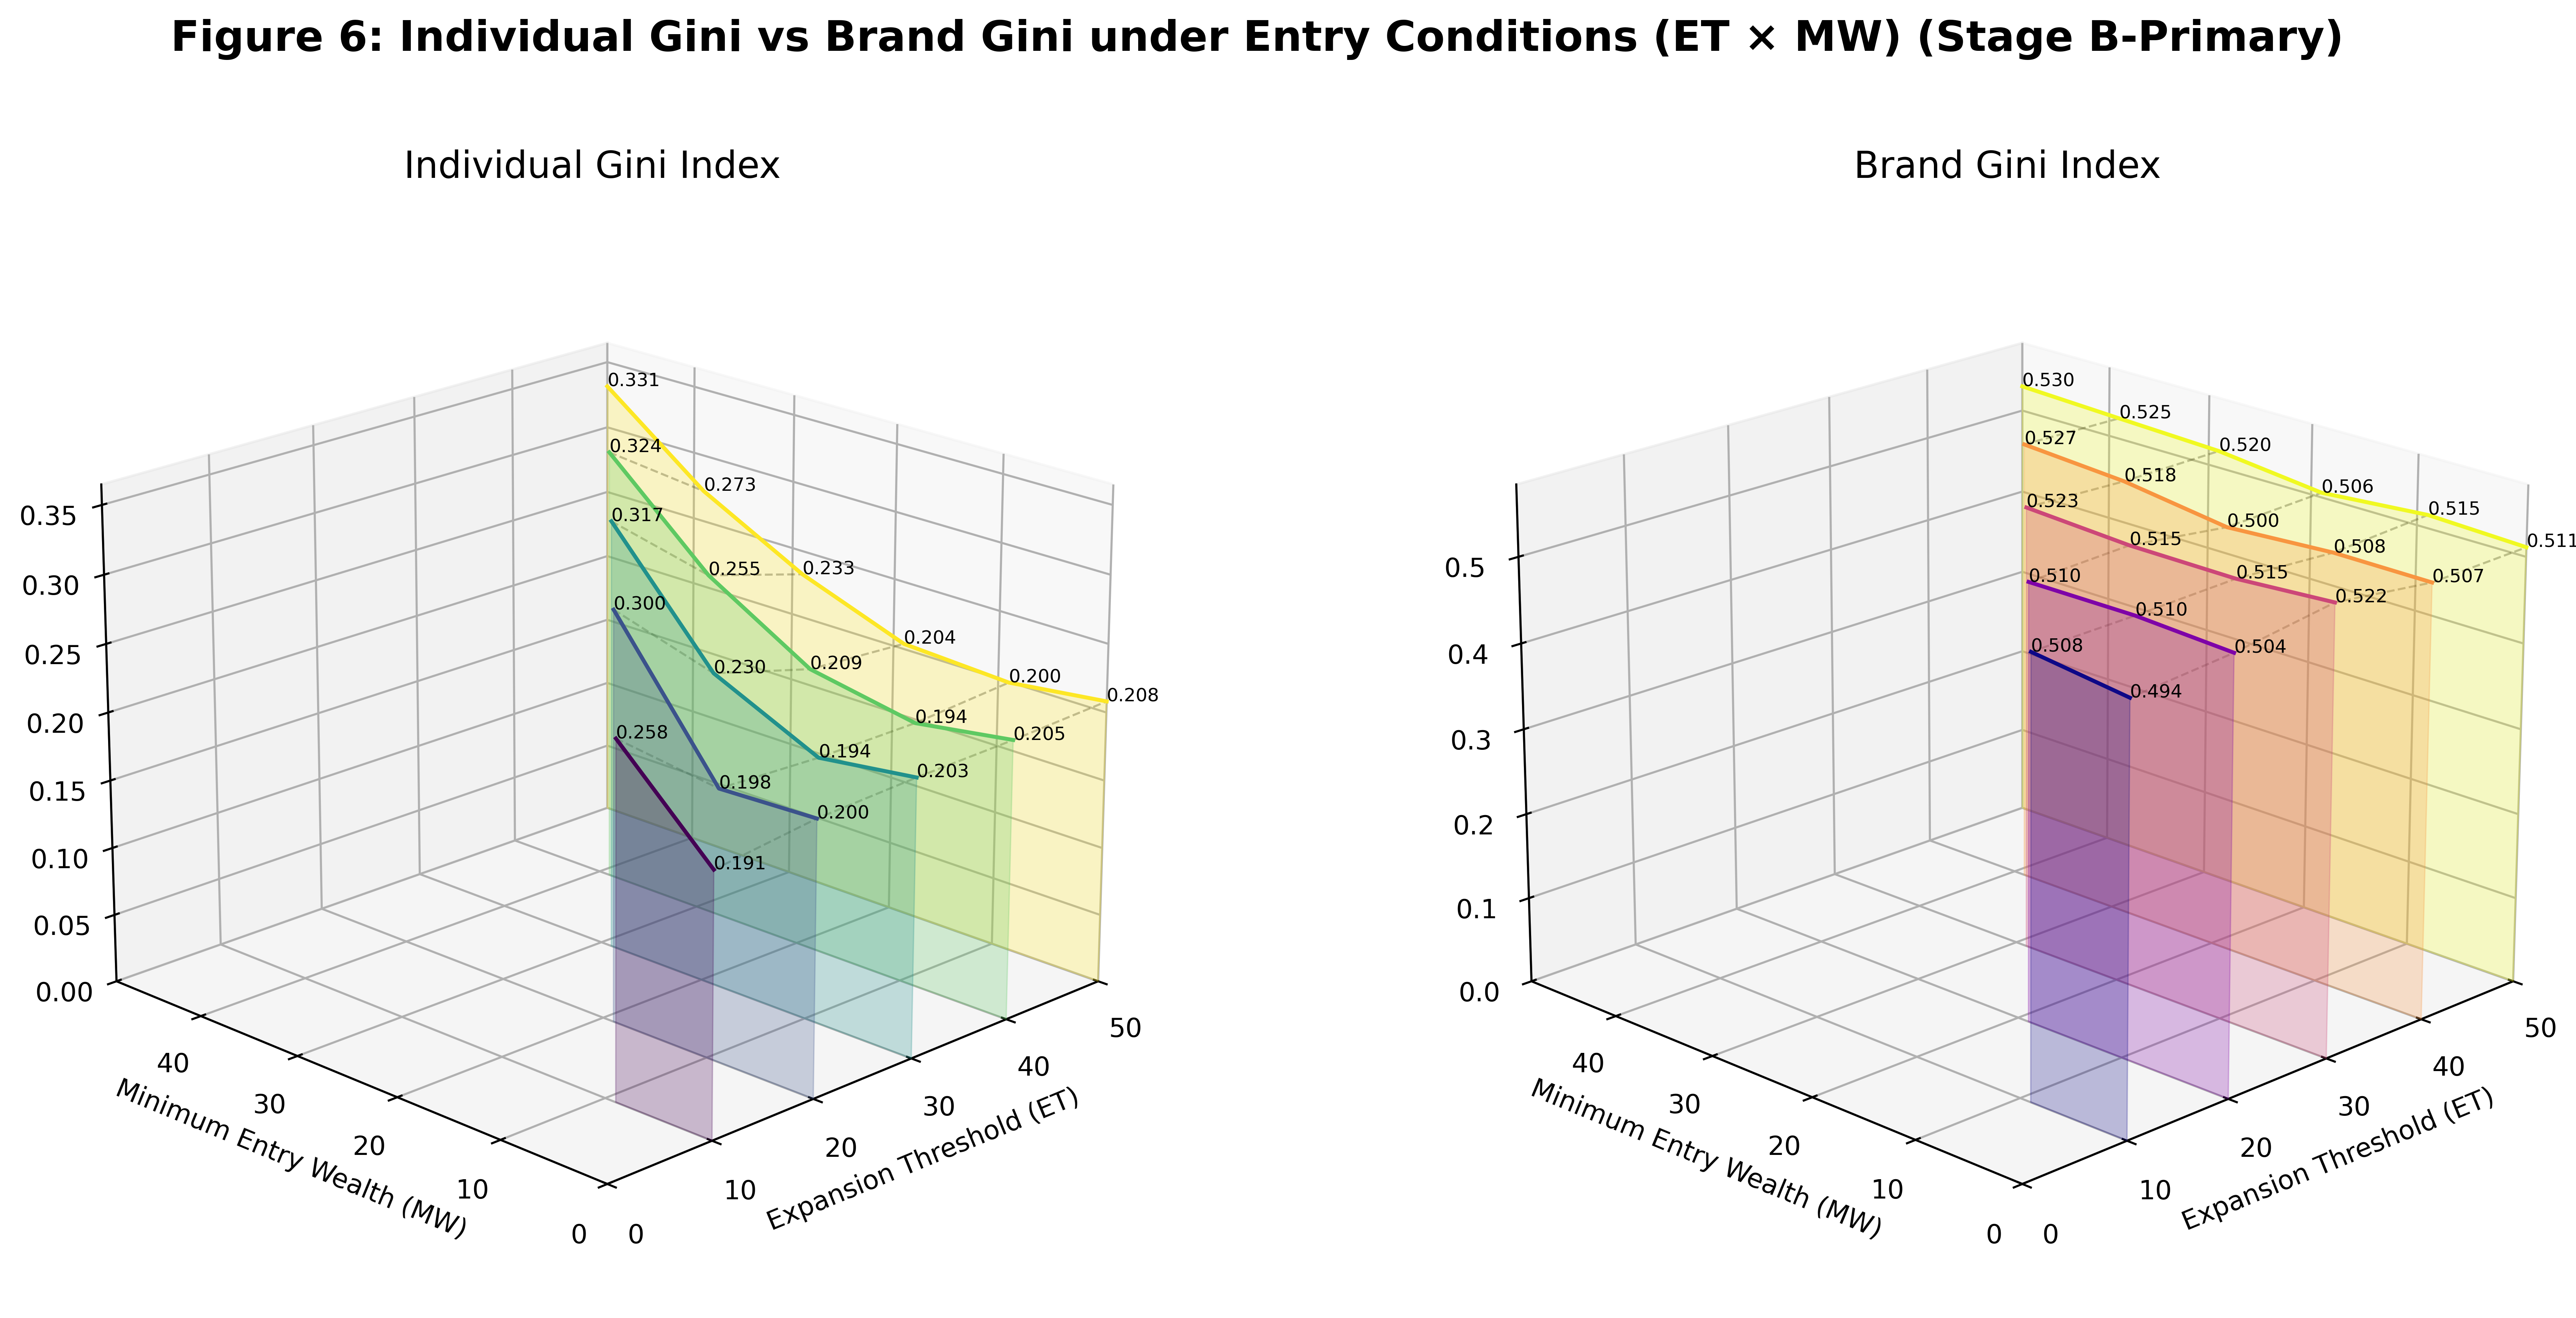
\includegraphics[width=0.75\linewidth]{stage_B_1_2.png}
\end{figure}

Figure 6 shows that individual Gini rises with MW (minimum entry wealth) and broadly declines with ET (expansion threshold). When the entry capital range $[\text{MW}, \text{ET}]$ narrows sharply, inequality intensifies further, peaking at 0.331 when ET $= 50$ and MW $= 49$. Brand Gini remains highly stable across all 20 valid combinations, ranging from 0.494 to 0.530.





\subsection{Stage B --- Secondary Experiment (Adjacency Harvest Bonus)}

\begin{figure}[H]
    \centering
    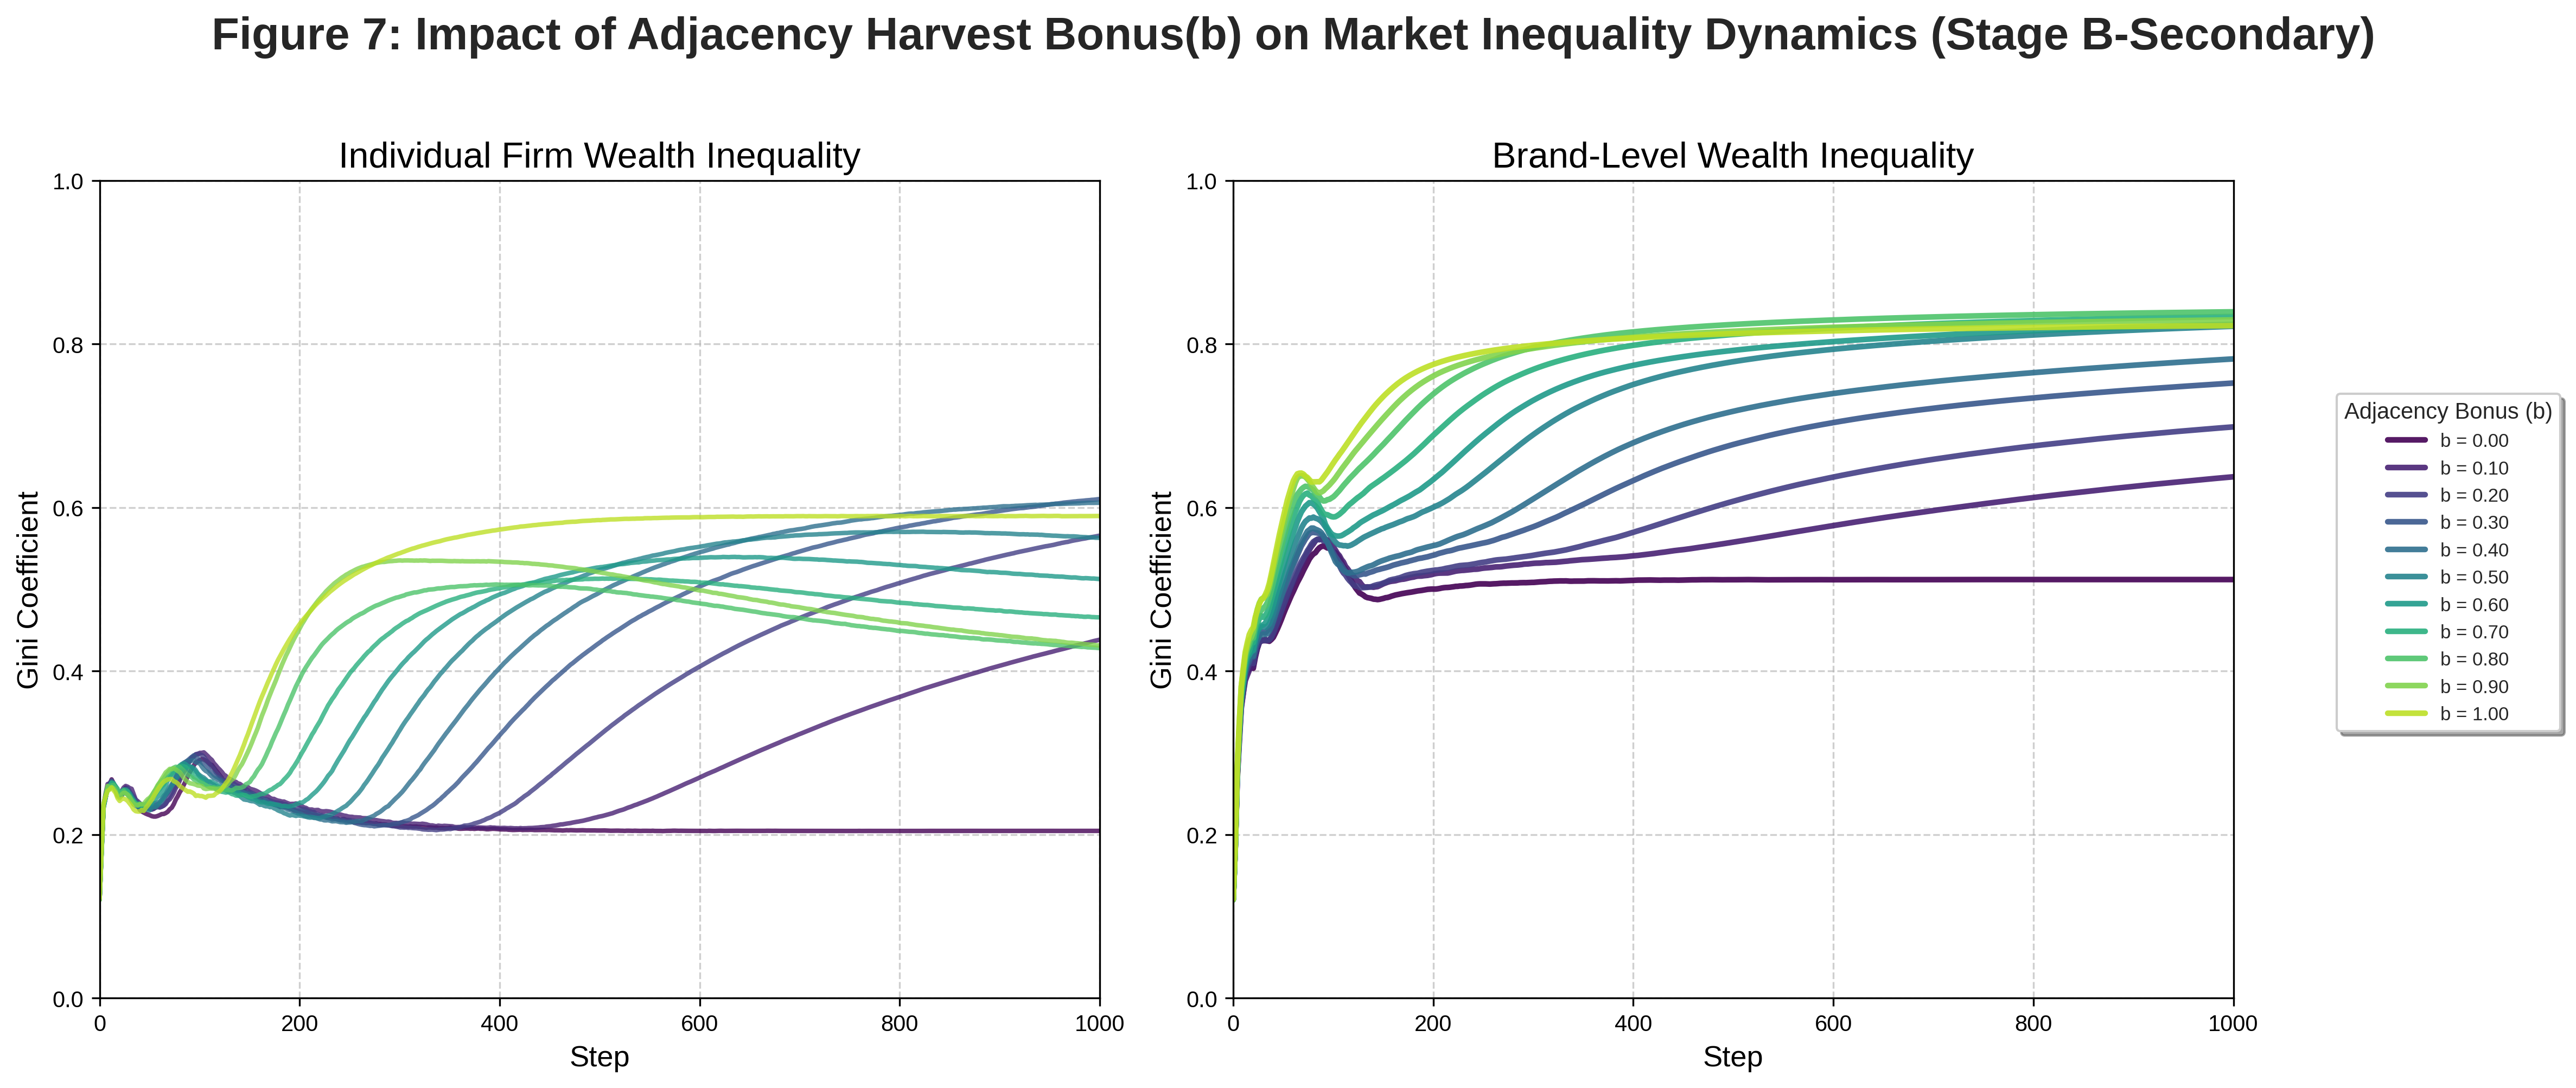
\includegraphics[width=1\linewidth]{stage_B_2_1.png}
\end{figure}

Figure 7 reveals contrasting patterns across the two Gini measures. Individual Gini rises from 0.205 at $b = 0$ to a peak of 0.610 at $b = 0.3$. It then declines to 0.428 at $b = 0.8$, before jumping again to 0.590 at $b = 1.0$. Brand Gini behaves differently. It jumps immediately from 0.512 to above 0.638 once $b > 0$, and continues rising to a peak of 0.839 when $b = 0.8$.

\begin{figure}[H]
    \centering
    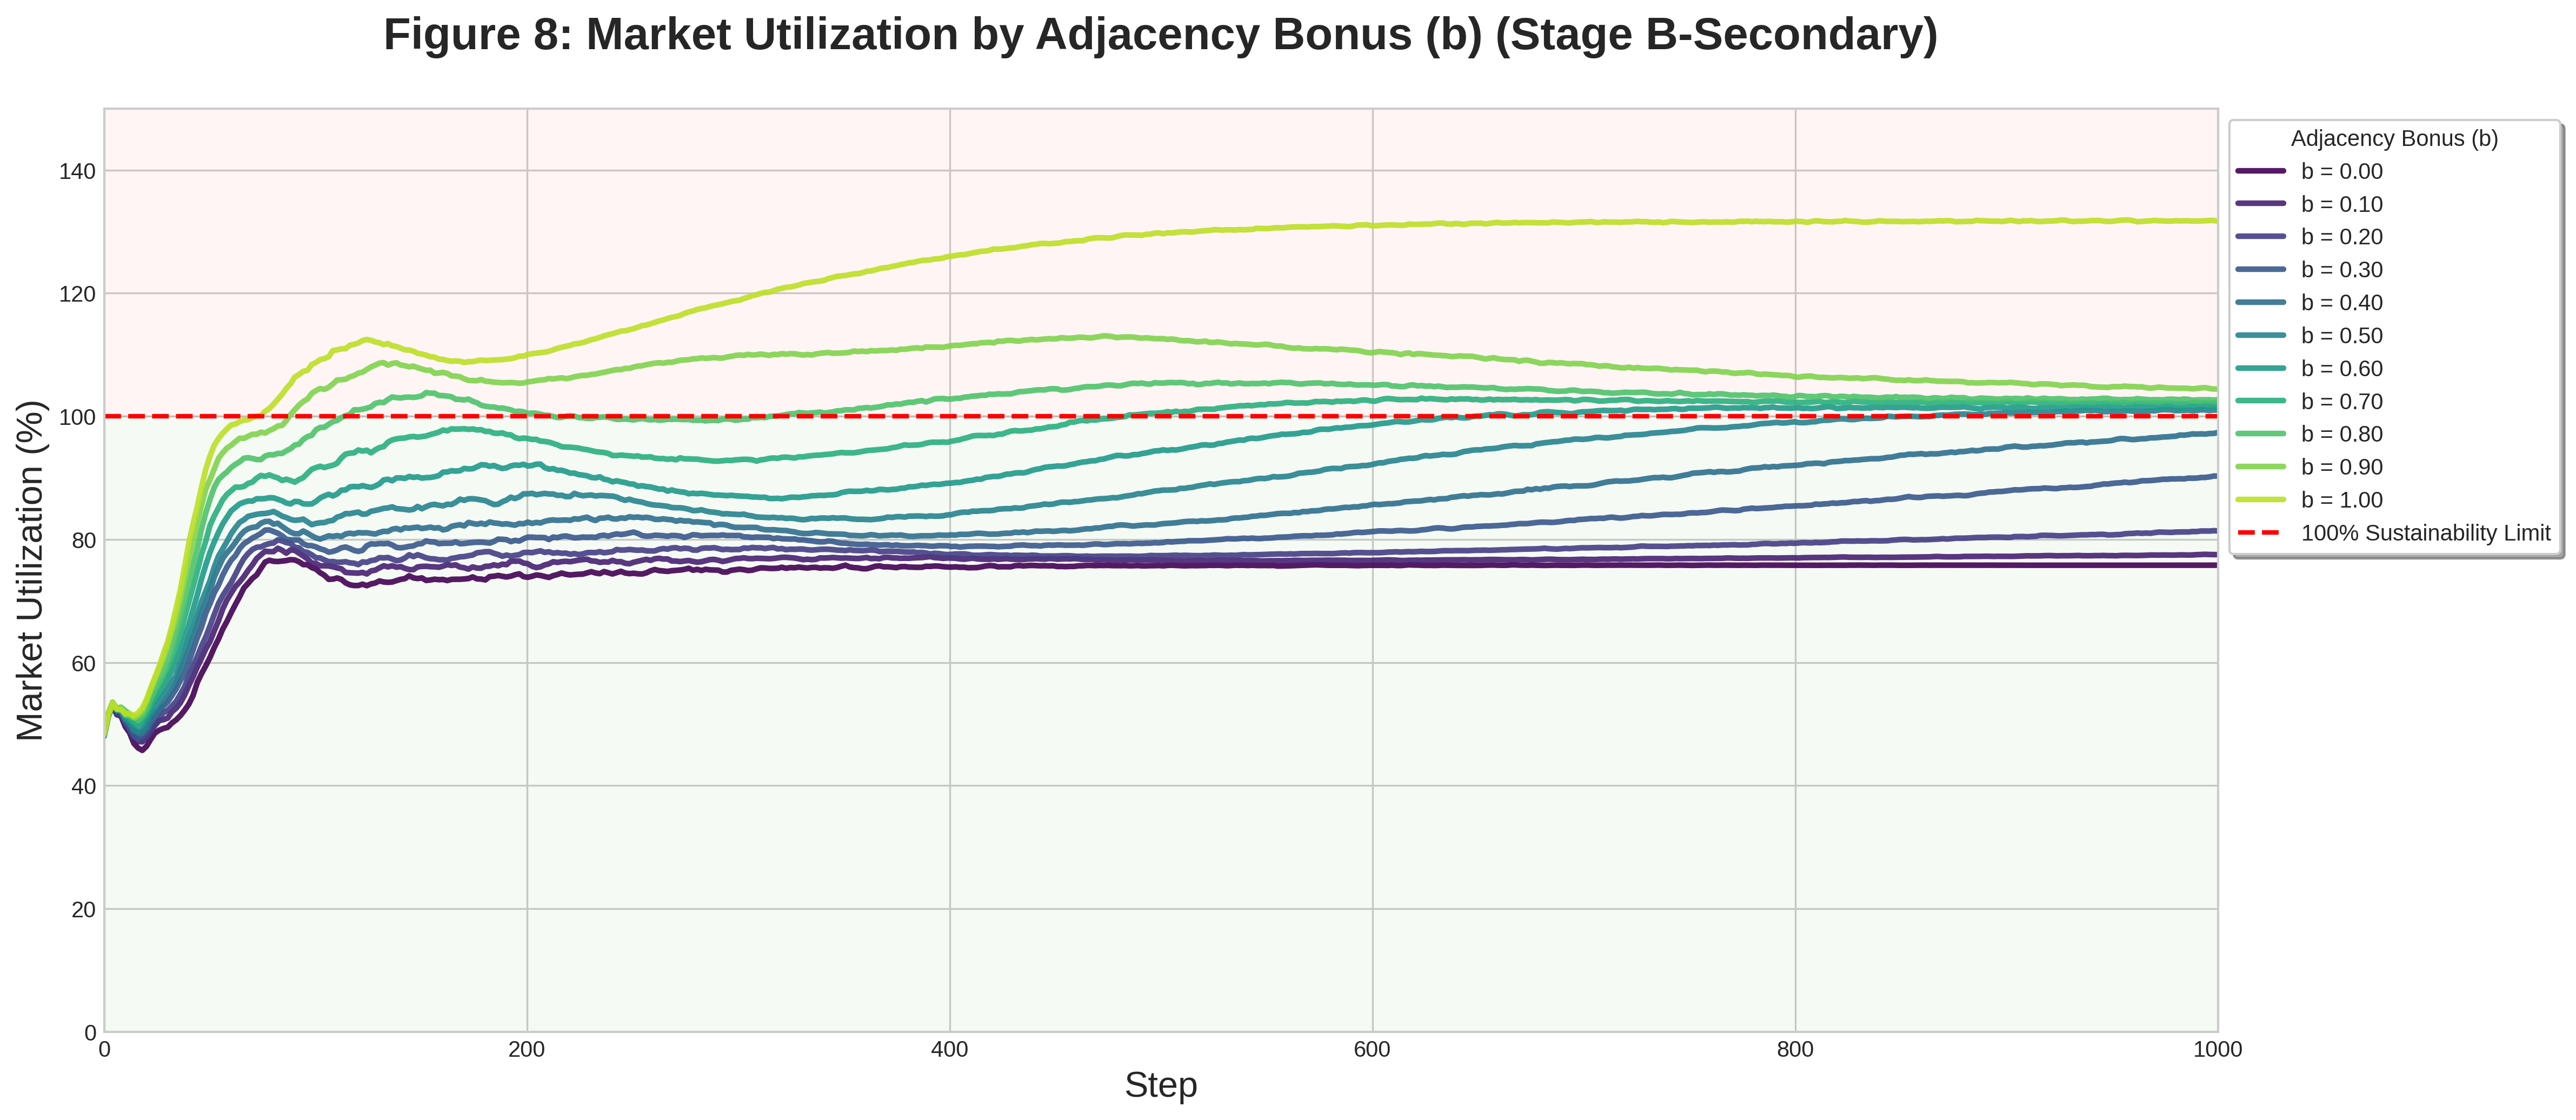
\includegraphics[width=1\linewidth]{stage_B_2_2.png}
\end{figure}

Figure 8 shows market utilization rising steadily with $b$. It first exceeds 100\% at $b = 0.5$, reaching 131.7\% when $b = 1.0$. 

% ============================================================
% 4. DISCUSSION
% ============================================================
\section{Discussion}

\subsection{Asymmetric Selection: Cost Over Awareness}
Both stages show that operating cost declines significantly under competitive pressure, while market reach remains relatively stable, indicating that high-cost firms are the first to go bankrupt and positional advantages are weakened as demand-rich patches become occupied in dense markets. 

\subsection{Structural Changes in Market Utilization}

Stage A’s utilization ceiling of approximately $47\%$ is independent of firm count, suggesting it is determined by the spatial distribution of market demand and the rate of demand renewal (sugar regeneration rate) in static market. In the Stage B primary experiment, the expansion mechanism stabilises utilization at $75.5\%$. when the adjacent harvest bonus is introduced, utilization exceeds $100\%$ and ultimately reaches $131.7\%$ as bonus rate increases. These jointly confirm a more scaled firm composition will drive expansion of market carrying capacity.


\subsection{Decoupling of Two Forms of Inequality}

In the Stage B primary experiment, when ET and MW are close in value, parent companies give homogeneous money for new firms as their startup capital. Thus the competition produces more polarised results at the aggregate level. Conversely, the wider capital range introduces heterogeneity, reducing individual-level inequality. Brand Gini remains approximately $0.51$, confirming that although the expansion mechanism reduces individual-level inequality, it introduces a higher level of inequality at the brand level.

\subsection{The Cross-Stage Decisive Role of Pre-Entry Market Intelligence}

The wide standard deviation bands at low density in Stage A indicate the importance of occupying resource-rich locations upon entry. It exerts significantly greater influence on individual outcomes than operational traits. In Stage B, the transmission of geographic advantage across generations enables dominant brands to accumulate wealth rapidly and becomes a structural source of brand-level inequality. The adjacency harvest bonus further amplifies this mechanism. Economies of scale raise clusters’ efficiency, and a positive feedback loop pushes brand Gini to its extreme peak of $0.839$. 




% 5. CONCLUSION
% ============================================================
\section{Conclusion}

This study examines how competitive pressure and market structure jointly shape firm survival and wealth inequality across stages. In the static market, the selection mechanism eliminates high-cost firms first, not those with weaker market awareness. In the dynamic expansion market, entry capital conditions: expansion threshold and minimum entry wealth affect individual-level inequality through the startup capital range. Brand-level wealth divergence, however, originates from random geographic positioning upon entry and compounds across generations as branches inherit locational advantage, which entry capital cannot offset. When the adjacency harvest bonus is introduced, scale efficiency further raises market carrying capacity and reinforces the positive feedback loop of geographic first-mover advantage, driving extreme brand-level inequality. The results also suggest that for firms and brands cost control is determinant of survival and intelligence in occupying demand-rich locations upon entry is fundamental to success.

% ============================================================
% REFERENCES
% ============================================================
\newpage
\begin{thebibliography}{99}

\bibitem{epstein1996}
Epstein, J. M. and Axtell, R. (1996)
\textit{Growing Artificial Societies: Social Science from the Bottom Up}.
MIT Press.

\bibitem{wilensky1999a}
Wilensky, U. (1999a)
\textit{NetLogo Models Library: Sugarscape 2 Constant Growback}.
Evanston, IL: Center for Connected Learning and Computer-Based Modeling,
Northwestern University.
Available at: \url{https://ccl.northwestern.edu/netlogo/models/Sugarscape2ConstantGrowback}

\bibitem{wilensky1999b}
Wilensky, U. (1999b)
\textit{NetLogo Models Library: Sugarscape 3 Wealth Distribution}.
Evanston, IL: Center for Connected Learning and Computer-Based Modeling,
Northwestern University.
Available at: \url{https://ccl.northwestern.edu/netlogo/models/Sugarscape3WealthDistribution}

\bibitem{park2024}
Park, D., Hong, J. and Ryu, D. (2024)
`Heterogeneous expectations in the housing market: a sugarscape agent-based model',
\textit{Journal of Housing and the Built Environment}, 39, pp. 1465--1489.

\end{thebibliography}




% ============================================================
% APPENDIX
% ============================================================
\newpage
\section*{Appendix}


\addcontentsline{toc}{section}{Appendix}

\subsection*{A. Stage A: Extended Code Chunk Based on Sugarscape Model 2}
% Description with Hyperlink
\noindent The complete model of \textbf{Stage-A: Static-Competitive-Market}, can be found in the following repository:

\vspace{0.5em}
\noindent \url{https://github.com/zhengpei-xu/CASA/blob/main/CASA0011_Agent-based-Modelling-for-Spatial-Systems/Coursework-1_Analysing-Models/Models/Stage-A_Static-Competitive-Market.nlogo}

\vspace{1.5em}

\begin{lstlisting}[language=NetLogo, caption={Reporter for market-utilization}]
;; -------------------addition part 1---------------------
;; ------------reportor for market-utilization------------
to-report get-market-utilization
  ;; 1. calculating the total metabolism of agents (total cost every tick)
  let total-demand sum [metabolism] of turtles
  
  ;; 2. caculating total Theoretical Maximum output (potential total market output)
  ; because the potential recovery value of each sugar mine is 1/tick
  ; now can use the number of mines to represent potential total market output (2069)
  let total-supply count patches with [max-psugar > 0]
  
  ; solving Zero Division Error
  if total-supply = 0 [report 0]

  ;; 3. reporting percentage
  report (total-demand / total-supply) * 100

end
\end{lstlisting}




\begin{lstlisting}[language=NetLogo, caption={Reporter for Gini Index}]
;; -------------------addition part 2--------------------
;; ------plot for Gini Index for wealth distribution-----
to update-lorenz-and-gini
  let num-people count turtles
  let sorted-wealths sort [sugar] of turtles
  let total-wealth sum sorted-wealths
  let wealth-sum-so-far 0
  let index 0
  set gini-index-reserve 0
  set lorenz-points []
  repeat num-people [
    set wealth-sum-so-far (wealth-sum-so-far + item index sorted-wealths)
    set lorenz-points lput ((wealth-sum-so-far / total-wealth) * 100) lorenz-points
    set index (index + 1)
    set gini-index-reserve
      gini-index-reserve +
      (index / num-people) -
      (wealth-sum-so-far / total-wealth)
  ]
end
\end{lstlisting}



\begin{lstlisting}[language=NetLogo, caption={Optional addition for brands property}]
;; -------------------addition part 3---------------------
;; ----------------adding brands property-----------------
;; -------------------this is optional--------------------
;;--------------just for aesthetic purposes---------------
to distribute-brands
  ;; Create the initial population based on the UI slider
  create-turtles initial-population [
    ;; Assign the unique 'who' number as the Brand ID 
    set brand who 
    
    ;; Set a unique color based on the Brand ID to visualize diversity
    ;; The modulo operator ensures colors stay within the NetLogo visible range.
    ;; Gemini used here to asign color
    set color (5 + (brand * 13) mod 135) 
    
    ;; Call the general turtle setup for traits and positioning
    turtle-setup
  ]
end
\end{lstlisting}












\subsection*{B. Stage B: Extended Code Chunk Based on Sugarscape Model 3}

% Description with Hyperlink
\noindent The complete model of \textbf{Stage B: Dynamic Expansion Market}, can be found in the following repository:

\vspace{0.5em}
\noindent \url{https://github.com/zhengpei-xu/CASA/blob/main/CASA0011_Agent-based-Modelling-for-Spatial-Systems/Coursework-1_Analysing-Models/Models/Stage-B_Dynamic-Expansion-Market.nlogox}

\vspace{1.5em}


\begin{lstlisting}[language=NetLogo, caption={Introduction of brands property}]
;; -------------------addition part 1---------------------
;; ----------------adding brands property-----------------
to distribute-brands
  ;; Create the initial population based on the UI slider
  create-turtles initial-population [
    ;; Assign the unique 'who' number as the Brand ID 
    set brand who 
    
    ;; Set a unique color based on the Brand ID to visualize diversity
    ;; The modulo operator ensures colors stay within the NetLogo visible range.
    ;; Gemini used here to asign color
    set color (5 + (brand * 13) mod 135) 
    
    ;; Call the general turtle setup for traits and positioning
    turtle-setup
  ]
end
\end{lstlisting}




\begin{lstlisting}[language=NetLogo, caption={Introduction of new expansion mechanism}]
;; -------------------addition part 2---------------------
;; ----------introducing new expansion mechanism----------
to handle-life-cycle ;; turtle procedure
  ;; 1. Initialize Expansion Cost
  let birth-cost random-in-range minimum-sugar-endowment maximum-sugar-endowment
  
  ;; --- 2. ACTIVE EXPANSION  ---
  ;; Prudence Check!!! Ensure expansion doesn't bankrupt the parent 
  if (sugar > maximum-sugar-endowment) and (not first-tick?) [
    
    ;; Safety Buffer: Assets after cost must exceed 1 tick of metabolism
    if (sugar - birth-cost > metabolism) [
      let target-patch one-of neighbors4 with [not any? turtles-here]
      
      if (random-float 1.0 < birth-rate) and (target-patch != nobody) [
        set sugar (sugar - birth-cost)
        
        hatch 1 [
          ;; inherit 'brand', but reset capabilities 
          turtle-setup      
          set sugar birth-cost
          ; first-tick protection buff
          set first-tick? true
          move-to target-patch
        ]
      ]
    ]
  ]
  
  ;; --- 3. STARVATION CHECK (Final Check) ---
  if sugar <= 0 [
    die 
  ]
  
  if first-tick? [ set first-tick? false ]
end
\end{lstlisting}



\begin{lstlisting}[language=NetLogo, caption={Addition of adjacency harvest bonus}]
;; -------------------addition part 3---------------------
;; ------------adding adjacency harvest bonus-------------
to turtle-eat ;; turtle procedure
  ;; 1. Check for same-brand neighbours in the four cardinal directions (up/down/left/right)
  let my-brand brand
  let allies-nearby (turtles-on neighbors4) with [brand = my-brand]
  
  ;; 2. Determine if a bonus should be applied
  let collection-amount psugar
  
  if any? allies-nearby [
    ;; Applying a bonus if at least one same-brand neighbour is directly adjacent
    set collection-amount (psugar * (1 + efficiency-gain))
  ]
  
  ;; 3. Update sugar storage (subtract metabolism + add boosted collection)
  set sugar (sugar - metabolism + collection-amount)
  
  ;; 4. Set patch sugar to 0 after consumption
  set psugar 0
end
\end{lstlisting}







\begin{lstlisting}[language=NetLogo, caption={Reporter for market-utilization}]
;; -------------------addition part 4---------------------
;; ------------reporter for market-utilization------------
to-report get-market-utilization
  ;; 1. calculating the total metabolism of agents (total cost every tick)
  let total-demand sum [metabolism] of turtles
  
  ;; 2. caculating total Theoretical Maximum output (potential total market output)
  ; because the potential recovery value of each sugar mine is 1/tick
  ; now can use the number of mines to represent potential total market output (2069)
  let total-supply count patches with [max-psugar > 0]
  
  ; solving Zero Division Error
  if total-supply = 0 [report 0]

  ;; 3. reporting percentage
  report (total-demand / total-supply) * 100

end
\end{lstlisting}


\begin{lstlisting}[language=NetLogo, caption={Reporter for Brand level Gini Index}]
;; -------------------addition part 5--------------------
;; ----plot for Brand Gini Index for brand inequality----
to update-brand-lorenz-and-gini
  let alive-brand-ids remove-duplicates [brand] of turtles
  let brand-wealths map [ b -> sum [sugar] of turtles with [brand = b] ] alive-brand-ids
  set num-brands length brand-wealths
  

  
  let sorted-wealths sort brand-wealths
  let total-wealth sum sorted-wealths
  
  if total-wealth = 0 [ stop ]
  
  let wealth-sum-so-far 0
  let index 0
  set brand-gini-index-reserve 0    
  set brand-lorenz-points []        
  
  repeat num-brands [
    set wealth-sum-so-far (wealth-sum-so-far + item index sorted-wealths)
    ;; Updating brand-specific lorenz list 
    set brand-lorenz-points lput ((wealth-sum-so-far / total-wealth) * 100) brand-lorenz-points
    set index (index + 1)
    ;; Calculating the specific reserve for brands
    set brand-gini-index-reserve
      brand-gini-index-reserve +
      (index / num-brands) -
      (wealth-sum-so-far / total-wealth)
  ]
end
\end{lstlisting}

















\end{document}




